\chapter{Diseño técnico}

En este capítulo analizaremos los requisitos de la aplicación previamente al inicio de su implementación.

\section{Listado de historias de usuario (\textit{Backlog})}

En el \textit{Backlog} vamos a incluir una lista de todo el trabajo necesario ordenado por prioridades a partir de la hoja de ruta que contiene los requisitos del producto \cite{whatIsBacklog}.

Para extraer las historias de usuario se ha usado la aplicación \textbf{Jira}\footnote{\url{https://www.atlassian.com/software/jira}}, de la compañía \textbf{Atlassian}. Por consistencia y aunque puedan parecer desordenados, los identificadores de las épicas y de las historias que aparecen en esta sección son los que se han obtenido en dicha herramienta.

En la figura \ref{fig:jiraBacklog} se puede observar la interfaz de usuario de \textbf{Jira} que se ha usado para registrar las historias de usuario. Así mismo, en la figura \ref{fig:jiraTodos} se puede observar el \textit{Backlog} completo exportado desde \textbf{Jira}.

\begin{figure}[h]
\centering
\captionsetup{justification=centering}
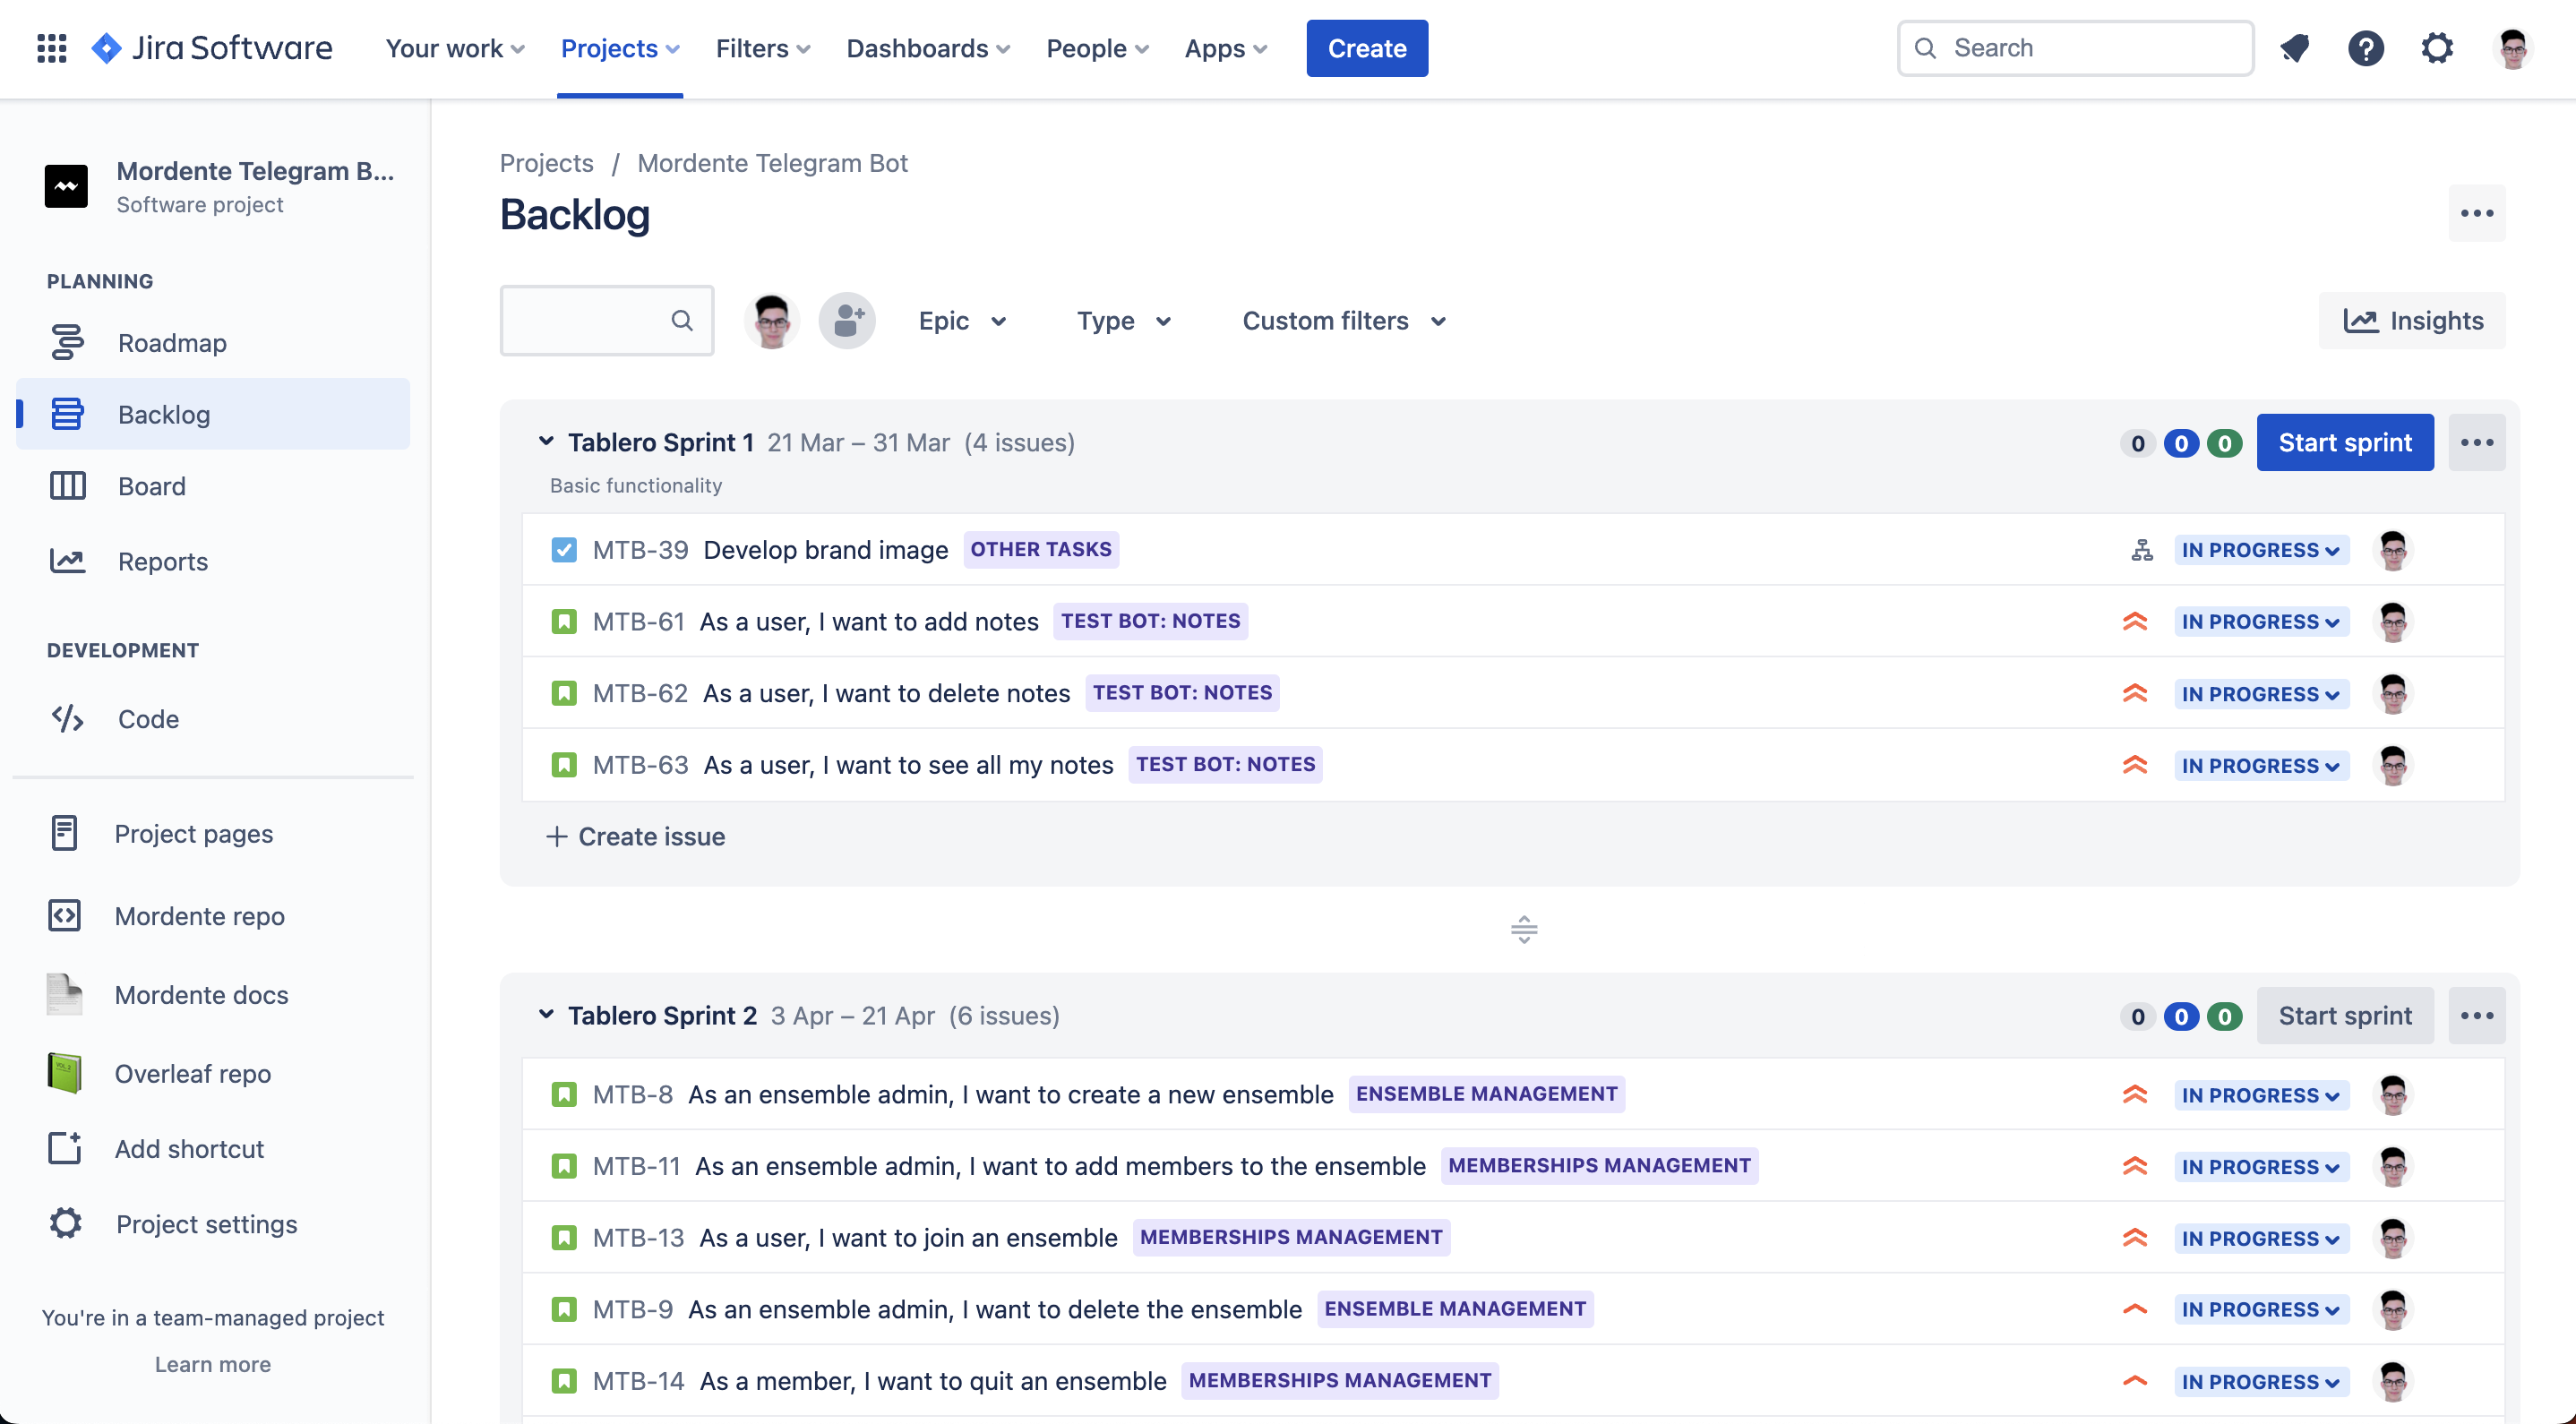
\includegraphics[width=\textwidth]{imagenes/disenyo_tecnico/jira_backlog.png}
\caption{Interfaz para crear y consultar historias de usuario en el \textit{Backlog} de \textbf{Jira}.}
\label{fig:jiraBacklog}
\end{figure}

\begin{figure}[h]
\centering
\captionsetup{justification=centering}
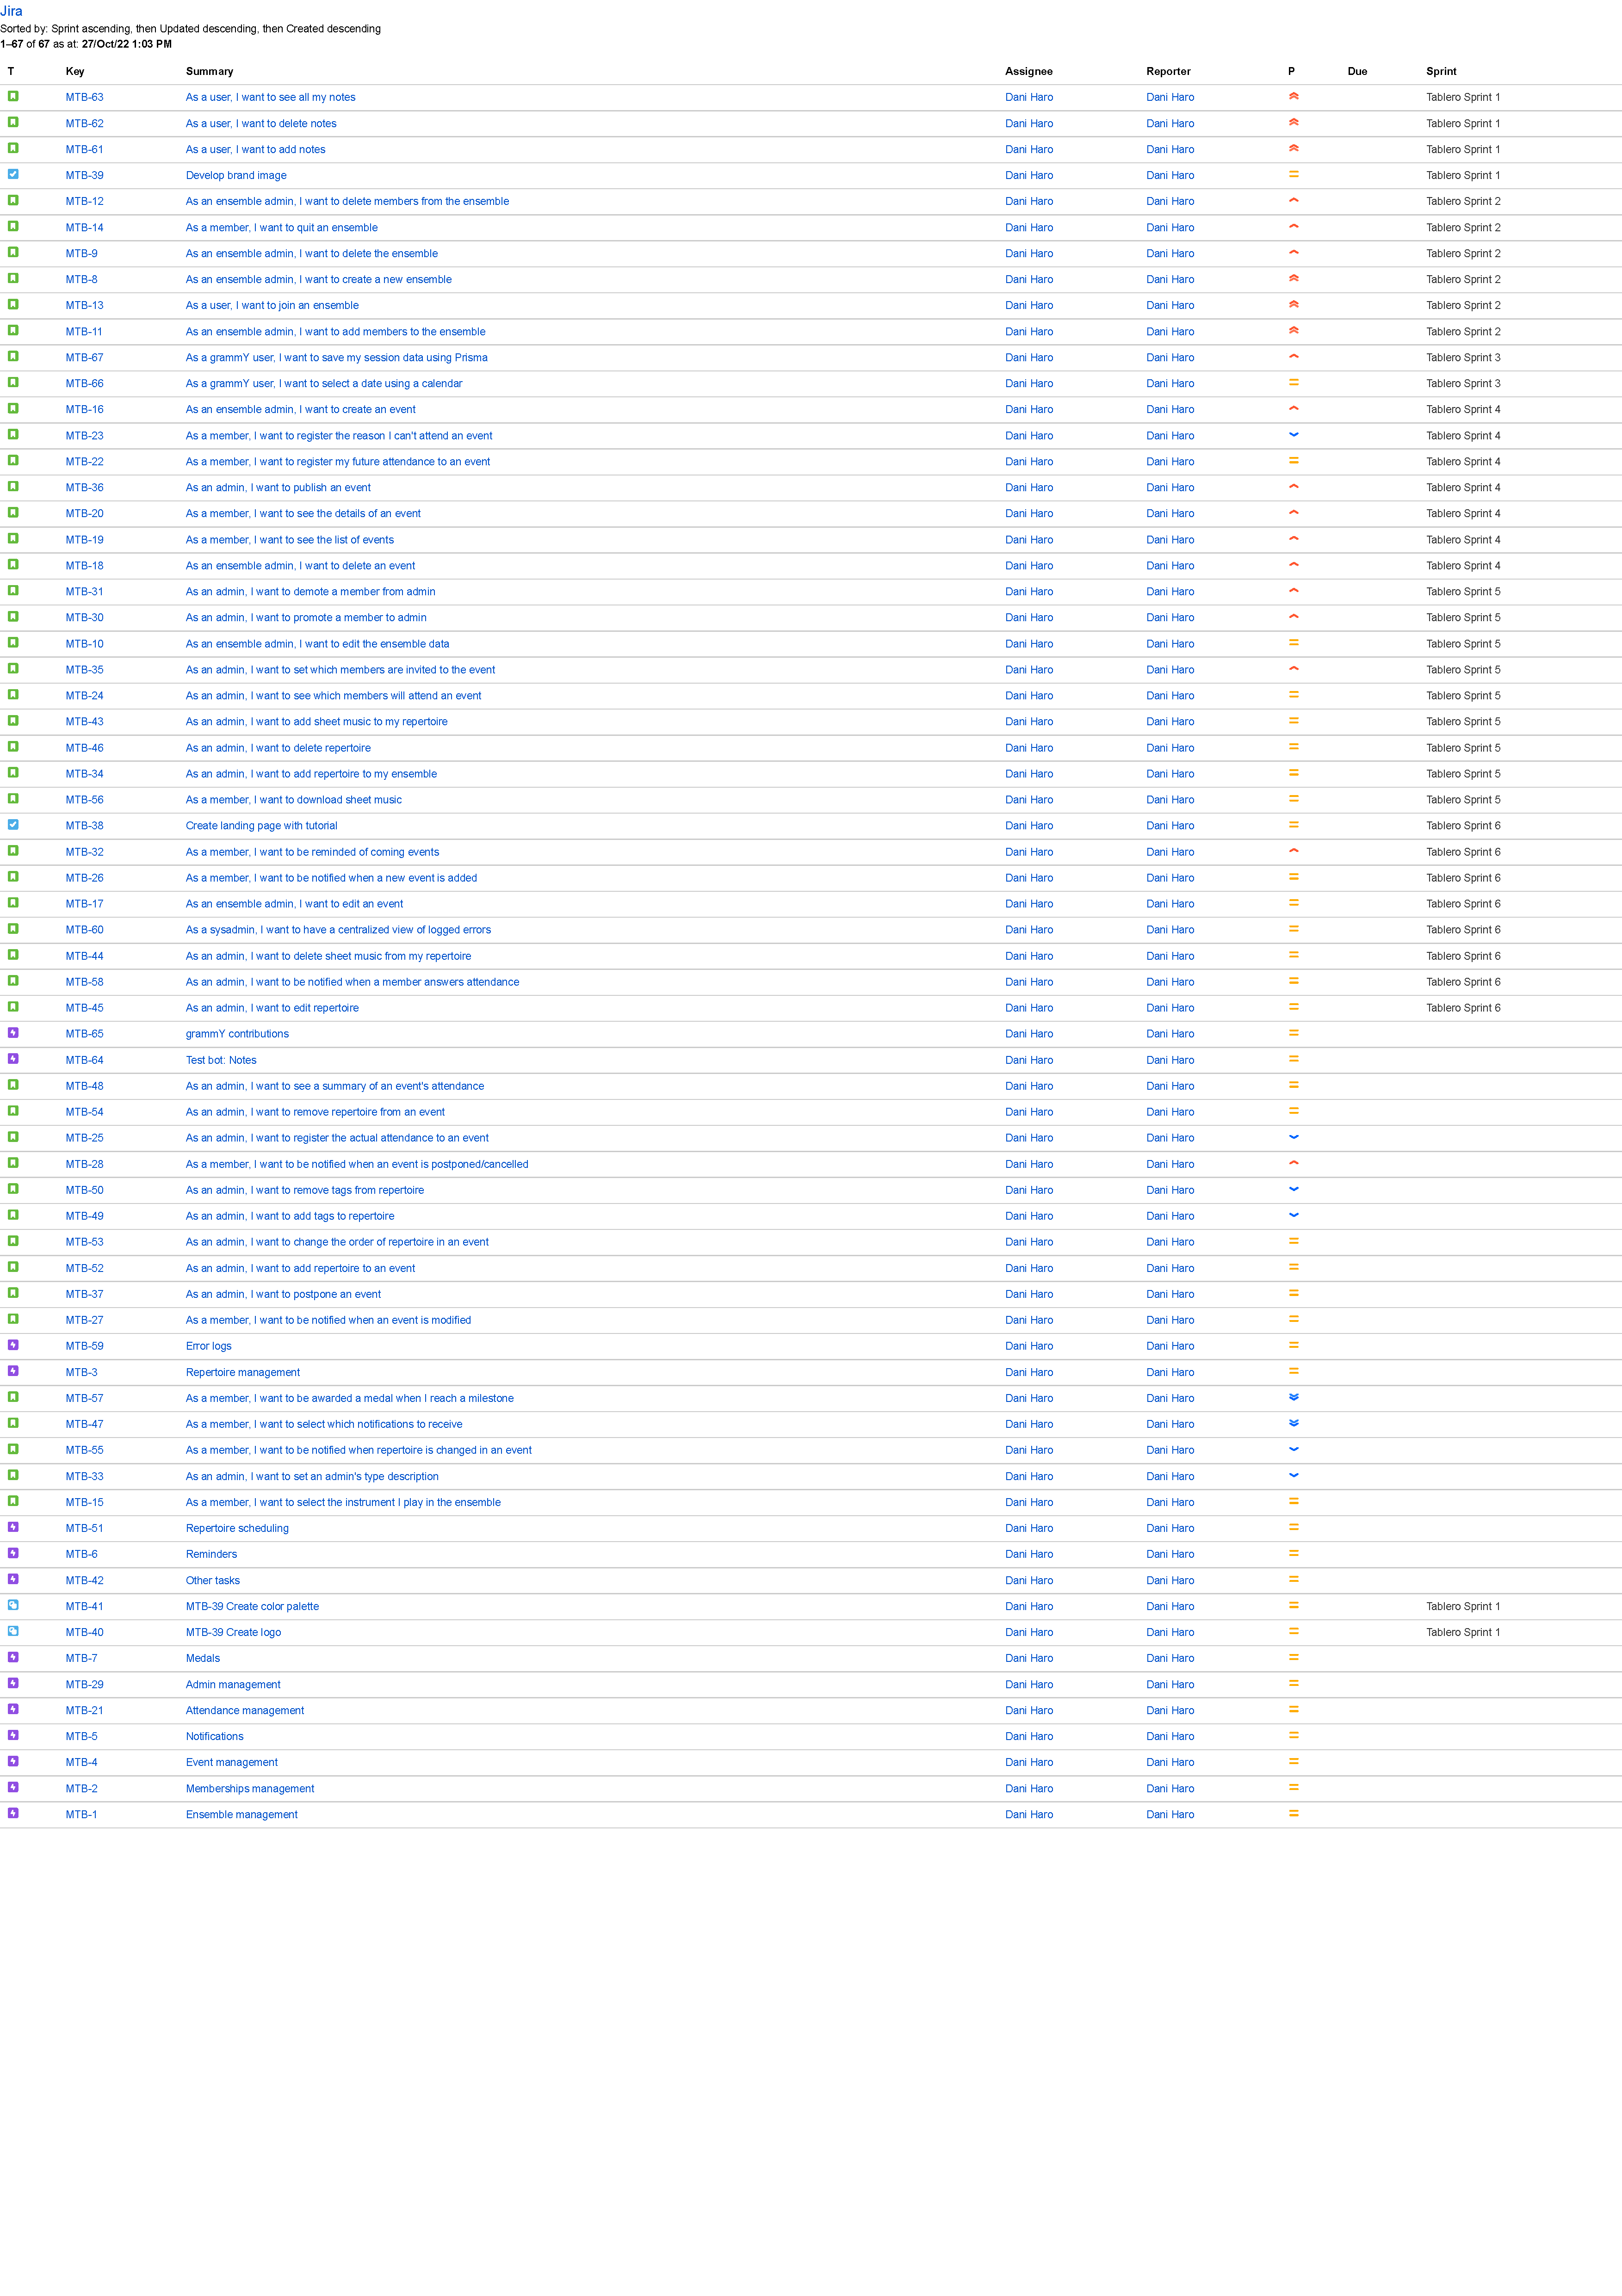
\includegraphics[width=\textwidth]{imagenes/disenyo_tecnico/jira_todos.pdf}
\caption{Lista completa de las historias de usuario creadas en el \textit{Backlog} de \textbf{Jira}.}
\label{fig:jiraTodos}
\end{figure}

A continuación vamos a mostrar las historias del backlog divididas en \textbf{épicas}, sin priorizar. Las \textbf{épicas} agrupan las historias de usuario dependiendo de qué parte de la lógica de negocio de la aplicación las relaciona.

\begin{enumerate}
    \item[MTB-64.] Bot de prueba: Notas.
        \begin{enumerate}
            \item[MTB-61.] Como usuario, quiero añadir notas.
            \item[MTB-62.] Como usuario, quiero eliminar una nota.
            \item[MTB-63.] Como usuario, quiero ver todas mis notas.
        \end{enumerate}
    \item[MTB-1.] Gestión de agrupaciones.
        \begin{enumerate}
            \item[MTB-8.] Como administrador de una agrupación, quiero crear una nueva agrupación.
            \item[MTB-9.] Como administrador de una agrupación, quiero eliminar mi agrupación.
            \item[MTB-10.] Como administrador de una agrupación, quiero editar mi agrupación.
        \end{enumerate}
    \item[MTB-2.] Gestión de membresías.
        \begin{enumerate}
            \item[MTB-11.] Como administrador de una agrupación, quiero añadir miembros a mi agrupación.
            \item[MTB-13.] Como usuario, quiero unirme a una agrupación.
            \item[MTB-12.] Como administrador de una agrupación, quiero eliminar miembros de la agrupación.
            \item[MTB-14.] Como miembro, quiero salirme de una agrupación.
            \item[MTB-15.] Como miembro, quiero seleccionar qué instrumento toco en la agrupación.
        \end{enumerate}
    \item[MTB-4.] Gestión de eventos.
        \begin{enumerate}
            \item[MTB-16.] Como administrador de una agrupación, quiero añadir un evento.
            \item[MTB-35.] Como administrador de una agrupación, quiero configurar qué miembros están invitados a un evento.
            \item[MTB-17.] Como administrador de una agrupación, quiero editar los datos de un evento.
            \item[MTB-18.] Como administrador de una agrupación, quiero eliminar un evento.
            \item[MTB-19.] Como miembro, quiero ver la lista de eventos a los que estoy invitado.
            \item[MTB-20.] Como miembro, quiero ver los detalles de un evento.
            \item[MTB-36.] Como administrador, quiero publicar un evento.
            \item[MTB-37.] Como miembro, quiero posponer un evento.
        \end{enumerate}
    \item[MTB-5.] Notificaciones.
        \begin{enumerate}
            \item[MTB-58.] Como administrador, quiero ser notificado cuando un miembro registra su asistencia prevista a un evento.
            \item[MTB-26.] Como miembro, quiero ser notificado cuando soy invitado a un evento.
            \item[MTB-27.] Como miembro, quiero ser notificado cuando se modifica un evento.
            \item[MTB-28.] Como miembro, quiero ser notificado cuando se pospone un evento.
            \item[MTB-55.] Como miembro, quiero ser notificado cuando se añada nuevo repertorio.
            \item[MTB-47.] Como miembro, quiero seleccionar qué notificaciones recibo.
        \end{enumerate}
    \item[MTB-21.] Gestión de asistencia.
        \begin{enumerate}
            \item[MTB-22.] Como miembro, quiero registrar mi asistencia prevista a un evento.
            \item[MTB-23.] Como miembro, quiero justificar mi ausencia a un evento.
            \item[MTB-24.] Como administrador, quiero ver qué miembros asistirán a un evento.
            \item[MTB-25.] Como administrador, quiero registrar la asistencia real a un evento.
            \item[MTB-48.] Como administrador, quiero ver un resumen de la asistencia a un evento.
        \end{enumerate}
    \item[MTB-6.] Recordatorios.
        \begin{enumerate}
            \item[MTB-32.] Como miembro, quiero recibir recordatorios de los eventos próximos.
        \end{enumerate}
    \item[MTB-29.] Gestión de administradores.
        \begin{enumerate}
            \item[MTB-30.] Como administrador, quiero hacer que un miembro sea administrador.
            \item[MTB-31.] Como administrador, quiero quitarle a un miembro los permisos de administrador.
            \item[MTB-33.] Como administrador, quiero especificar mi rol como administrador.
        \end{enumerate}
    \item[MTB-3.] Gestión de repertorio.
        \begin{enumerate}
            \item[MTB-34.] Como administrador, quiero añadir repertorio a mi agrupación.
            \item[MTB-45.] Como administrador, quiero editar una obra.
            \item[MTB-46.] Como administrador, quiero eliminar una obra.
            \item[MTB-43.] Como administrador, quiero añadir la partitura de una obra.
            \item[MTB-44.] Como administrador, quiero eliminar la partitura de una obra.
            \item[MTB-49.] Como administrador, quiero añadir un \textit{tag} a una obra.
            \item[MTB-50.] Como administrador, quiero eliminar un \textit{tag} de una obra.
            \item[MTB-56.] Como miembro, quiero descargar las partituras.
        \end{enumerate}
    \item[MTB-59.] Registro de errores.
        \begin{enumerate}
            \item[MTB-60.] Como administrador de sistemas, quiero tener una vista centralizada de los errores que se hayan registrado en la aplicación.
        \end{enumerate}
    \item[MTB-42.] Otras tareas.
        \begin{enumerate}
            \item[MTB-38.] Crear la \textit{landing page} del proyecto.
            \item[MTB-39.] Crear la imagen de marca.
        \end{enumerate}
\end{enumerate}


En la tabla \ref{tab:historiasPriorizadas} se muestran las historias priorizadas y divididas en los distintos \textit{sprints} que se han planificado.


\begin{longtable}{| p{.12\textwidth} | p{.58\textwidth} | p{.12\textwidth} | p{.08\textwidth} |}
\hline
ID & Título & Prioridad & Sprint \\ \hline
MTB-39 & Crear la imagen de marca & Alta & 1 \\ \hline
MTB-61 & Como usuario, quiero añadir notas & Muy alta & 1 \\ \hline
MTB-62 & Como usuario, quiero eliminar notas & Muy alta & 1 \\ \hline
MTB-63 & Como usuario, quiero ver mis notas & Muy alta & 1 \\ \hline
MTB-8 & Como administrador, quiero crear una agrupación & Muy alta & 2 \\ \hline
MTB-11 & Como administrador, quiero añadir miembros a mi agrupación & Muy alta & 2 \\ \hline
MTB-13 & Como usuario, quiero unirme a una agrupación & Muy alta & 2 \\ \hline
MTB-9 & Como administrador, quiero eliminar una agrupación & Alta & 2 \\ \hline
MTB-14 & Como miembro, quiero salir de una agrupación & Alta & 2 \\ \hline
MTB-12 & Como administrador, quiero eliminar miembros de mi agrupación & Alta & 2 \\ \hline
MTB-66 & Como programador de un bot, quiero que mis usuarios puedan seleccionar una fecha usando un calendario & Media & 3 \\ \hline
MTB-67 & Como programador de un bot, quiero guardar la sesión en \texttt{prisma} & Alta & 3 \\ \hline
MTB-16 & Como administrador, quiero crear un evento & Alta & 4 \\ \hline
MTB-19 & Como miembro, quiero ver la lista de eventos & Alta & 4 \\ \hline
MTB-20 & Como miembro, quiero ver el detalle de un evento & Alta & 4 \\ \hline
MTB-18 & Como administrador, quiero eliminar un evento & Alta & 4 \\ \hline
MTB-36 & Como administrador, quiero publicar un evento & Alta & 4 \\ \hline
MTB-22 & Como miembro, quiero registrar mi previsión de asistencia a un evento & Media & 4 \\ \hline
MTB-23 & Como miembro, quiero registrar por qué no puedo asistir a un evento & Baja & 4 \\ \hline
MTB-30 & Como administrador, quiero hacer que un miembro sea administrador & Alta & 5 \\ \hline
MTB-31 & Como administrador, quiero quitarle a un miembro los permisos de administrador & Alta & 5 \\ \hline
MTB-35 & Como administrador, quiero invitar a miembros a un evento & Alta & 5 \\ \hline
MTB-34 & Como administrador, quiero añadir repertorio a mi agrupación & Media & 5 \\ \hline
MTB-43 & Como administrador, quiero añadir la partitura de una obra & Media & 5 \\ \hline
MTB-56 & Como miembro, quiero descargar una partitura & Media & 5 \\ \hline
MTB-46 & Como administrador, quiero eliminar una obra & Media & 5 \\ \hline
MTB-24 & Como administrador, quiero ver qué miembros asistirán a un evento & Media & 5 \\ \hline
MTB-10 & Como administrador, quiero editar mi agrupación & Media & 5 \\ \hline
MTB-32 & Como miembro, quiero recibir recordatorios de los eventos diarios & Alta & 6 \\ \hline
MTB-26 & Como miembro, quiero recibir una notificación cuando se me invite a un evento & Media & 6 \\ \hline
MTB-17 & Como administrador, quiero editar un evento & Media & 6 \\ \hline
MTB-45 & Como administrador, quiero editar una obra & Media & 6 \\ \hline
MTB-58 & Como administrador, quiero recibir una notificación cuando un miembro conteste sobre su asistencia a un evento & Media & 6 \\ \hline
MTB-44 & Como administrador, quiero eliminar una partitura & Baja & 6 \\ \hline
MTB-60 & Como administrador de sistemas, quiero tener una vista centralizada de los errores registrados & Media & 6 \\ \hline
MTB-38 & Como usuario, quiero ver una página web con información sobre Mordente & Baja & 6 \\ \hline
\caption{Historias de usuario priorizadas}
\label{tab:historiasPriorizadas}
\end{longtable}


\section{Historias de usuario}

En esta sección describiremos en detalle cada una de las historias de usuario, incluyendo su \textbf{descripción}, las \textbf{pruebas de aceptación} necesarias para darla por completada y las \textbf{tareas} en las que se subdivide.

\setlist[itemize]{nosep, noitemsep, topsep=0pt}

\newcommand{\historia}[5]{
\begin{table}[H]
\setlength\extrarowheight{2pt} % for a bit of visual "breathing space"
\begin{tabularx}{\textwidth}{| p{.20\textwidth} | p{.73\textwidth} |}
\hline
\textbf{Identificador} & #1. #2  \\ \hline
\textbf{Descripción} & #3  \\ \hline
\textbf{Pruebas de aceptación} & #4  \\ \hline
\textbf{Tareas} & #5  \\ \hline
\end{tabularx}
\caption{Historia de usuario #1}\label{tab:mtb#1}
\end{table}
}

\historia{MTB-39}{Crear la imagen de marca}{Crear una imagen reconocible de la marca \textbf{Mordente}: logotipo y colores.}{
\begin{itemize}
    \item Ver el logotipo en la página web.
    \item Ver el logotipo en el bot.
    \item Ver los colores de marca en la página web.
\end{itemize}
}{
\begin{itemize}
    \item Añadir el logotipo a la web.
    \item Cambiar los colores de la web.
    \item Cambiar foto de perfil del bot.
\end{itemize}
}

\historia{MTB-61}{Como usuario, quiero añadir notas}{
Añadir notas al bot de prueba con el comando \texttt{/add}.
}{
\begin{itemize}
    \item Las notas se guardan con el formato en el que se enviaron.
    \item Las notas se guardan asignadas al usuario que las crea.
\end{itemize}
}{
\begin{itemize}
    \item Conectar bot con base de datos.
    \item Manejar el comando \texttt{/add}.
    \item Hacer petición a base de datos para añadir nota.
\end{itemize}
}

\historia{MTB-62}{Como usuario, quiero eliminar notas}{
Cada usuario podrá eliminar las notas que ha añadido.
}{
\begin{itemize}
    \item Si intento eliminar una nota que no existe, recibo un error.
\end{itemize}
}{
\begin{itemize}
    \item Manejar el comando \texttt{/delete}.
    \item Hacer petición a base de datos para eliminar nota.
\end{itemize}
}

\historia{MTB-63}{Como usuario, quiero ver mis notas}{
Cada usuario podrá ver las notas que ha añadido.
}{
\begin{itemize}
    \item No puedo ver las notas de otros usuarios.
    \item Veo las notas en el formato en el que las añadí.
\end{itemize}
}{
\begin{itemize}
    \item Consulta a base de datos.
    \item Manejar comando \texttt{/list}.
\end{itemize}
}

\historia{MTB-8}{Como administrador, quiero crear una agrupación}{
Los usuarios del bot podrán crear una nueva agrupación, convirtiéndose inmediatamente en su administrador.
}{
\begin{itemize}
    \item Cuando se ha creado la agrupación, soy su administrador.
\end{itemize}
}{
\begin{itemize}
    \item Manejar comando \texttt{/start}.
    \item Manejar comando \texttt{/create}.
\end{itemize}
}

\historia{MTB-11}{Como administrador, quiero añadir miembros a mi agrupación}{
Los administradores podrán invitar a usuarios a su agrupación mediante un enlace de invitación generado.
}{
\begin{itemize}
    \item Cuando recibo el enlace, puedo reenviarlo a un usuario.
    \item En cualquier momento puedo hacer que no se pueda usar ese enlace.
\end{itemize}
}{
\begin{itemize}
    \item Añadir vista de lista de agrupaciones.
    \item Añadir vista de detalle de agrupación.
    \item Añadir menú de agrupación, con botón de \texttt{Invitar}.
    \item Añadir botón de \texttt{Deshabilitar enlace} si está activado.
    \item Generar código para el enlace.
    \item Consulta a base de datos para saber si el usuario es administrador.
    \item Petición a base de datos para activar o desactivar enlace.
\end{itemize}
}

\historia{MTB-13}{Como usuario, quiero unirme a una agrupación}{
Los usuarios del bot podrán unirse a una agrupación abriendo un enlace que les haya proporcionado un administrador.
}{
\begin{itemize}
    \item Si abro un enlace que no existe, recibo un error.
    \item Si el enlace está deshabilitado, recibo un error.
    \item Si el enlace es correcto, recibo una confirmación y los detalles de la agrupación.
\end{itemize}
}{
\begin{itemize}
    \item Manejar comando \texttt{/start} acompañado del código de invitación.
    \item Petición a base de datos para comprobar que la agrupación existe y su enlace de invitación está activado.
    \item Petición a base de datos para añadir nueva membresía.
\end{itemize}
}

\historia{MTB-9}{Como administrador, quiero eliminar una agrupación}{
En el menú de una agrupación, los administradores podrán elegir eliminarla.
}{
\begin{itemize}
    \item Si no soy administrador, no puedo eliminar la agrupación.
    \item Al pulsar el botón, se solicita una confirmación.
    \item Si contesto que finalmente no quiero eliminar, no se elimina.
    \item Si contesto que sí quiero, se elimina la agrupación y todos sus datos relacionados.
\end{itemize}
}{
\begin{itemize}
    \item Implementar menú de agrupación.
    \item Implementar conversación para confirmar si desea seguir con la eliminación.
    \item Consulta a base de datos para saber si el usuario es administrador.
    \item Petición a base de datos para eliminar la agrupación.
    \item Confirmación de la eliminación.
\end{itemize}
}

\historia{MTB-14}{Como miembro, quiero salir de una agrupación}{
En el menú de membresía, cada miembro podrá elegir salir de la agrupación.
}{
\begin{itemize}
    \item Si me salgo de la agrupación, también se eliminan mis invitaciones a eventos.
\end{itemize}
}{
\begin{itemize}
    \item Menú de agrupación con botón para salirme de la agrupación.
    \item Petición a base de datos para eliminar la membresía.
\end{itemize}
}

\historia{MTB-12}{Como administrador, quiero eliminar miembros de mi agrupación}{
En el menú de membresía, los administradores podrán seleccionar la opción de \texttt{Eliminar miembro}.
}{
\begin{itemize}
    \item Si no soy administrador, no puedo realizar la acción.
    \item Cuando elimino un miembro, también se eliminan sus invitaciones a eventos.
\end{itemize}
}{
\begin{itemize}
    \item Menú de agrupación con botón para eliminar de la agrupación a un miembro.
    \item Consulta a base de datos para saber si el usuario es administrador.
    \item Petición a base de datos para eliminar la membresía.
\end{itemize}
}

\historia{MTB-66}{Como programador de un bot, quiero que mis usuarios puedan seleccionar una fecha usando un calendario}{
Se debe desarrollar un complemento para \texttt{grammY} que proporcione un selector de fechas a modo de calendario.
}{
\begin{itemize}
    \item No se puede seleccionar una fecha inferior a la marcada como mínima.
    \item No se puede seleccionar una fecha superior a la marcada como máxima.
\end{itemize}
}{
\begin{itemize}
    \item Implementar nuevo menú personalizado que guarda estado de la fecha.
    \item Implementar \texttt{middleware} que guarda en el contexto qué fecha se ha seleccionado cuando el usuario ha terminado la selección.
    \item Implementar opciones del calendario: fecha mínima, máxima, botones adicionales.
\end{itemize}
}

\historia{MTB-67}{Como programador de un bot, quiero guardar la sesión en \texttt{prisma}}{
Se debe desarrollar un paquete para \texttt{grammY} que permita guardar la sesión utilizando \texttt{prisma}, y publicarlo para el resto de la comunidad.
}{
\begin{itemize}
    \item El \textit{plugin} debe pasar todos los tests implementados en la biblioteca de adaptadores de sesión.
\end{itemize}
}{
\begin{itemize}
    \item Clonar repositorio de adaptadores de sesión en local.
    \item Crear nuevo adaptador para prisma tomando inspiración del de \texttt{TypeORM}.
    \item Implementar los tests.
    \item Iterar hasta que los tests tengan resultado positivo.
    \item Publicar el \textit{plugin}.
\end{itemize}
}

\historia{MTB-16}{Como administrador, quiero crear un evento}{
En la lista de eventos, los administradores verán la opción de crear un nuevo evento, lo cual abrirá una conversación para su creación.
}{
\begin{itemize}
    \item Si no soy administrador, no puedo realizar la acción.
    \item Puedo saltar los pasos opcionales.
    \item Si selecciono una fecha que no existe, recibo un error.
    \item Si selecciono una hora que no existe, recibo un error.
\end{itemize}
}{
\begin{itemize}
    \item Consulta a base de datos para saber si el usuario es administrador.
    \item Menú de lista de eventos.
    \item Botón de crear evento en lista de eventos.
    \item Conversación para crear el evento.
    \item Petición a base de datos para crear el evento.
\end{itemize}
}

\historia{MTB-19}{Como miembro, quiero ver la lista de eventos}{
Cada miembro podrá ver la lista de eventos a los que está asignado.
}{
\begin{itemize}
    \item Si no soy miembro de la agrupación no puedo ver los eventos.
    \item Si no estoy invitado a un evento, no puedo verlo en la lista.
\end{itemize}
}{
\begin{itemize}
    \item Consulta a base de datos de la lista de eventos para el miembro.
    \item Vista de lista de eventos.
\end{itemize}
}

\historia{MTB-20}{Como miembro, quiero ver el detalle de un evento}{
En la lista de eventos, los miembros podrán escoger un evento para ver sus detalles.
}{
\begin{itemize}
    \item Si no soy miembro de la agrupación no puedo ver el evento.
    \item Si el evento consultado no existe recibo un error.
\end{itemize}
}{
\begin{itemize}
    \item Manejar comando \texttt{/event\_N}
    \item Vista de detalle de evento.
    \item Consulta a base de datos del detalle del evento.
\end{itemize}
}

\historia{MTB-18}{Como administrador, quiero eliminar un evento}{
En el menú de un evento, los administradores verán una opción de eliminarlo.
}{
\begin{itemize}
    \item Si no soy administrador, no puedo realizar la acción.
    \item Si no participo en la agrupación, no puedo realizar la acción.
    \item Recibo una pregunta de confirmación de la eliminación.
    \item Si selecciono finalmente que no quiero eliminar, no se elimina el evento.
    \item Al eliminar el evento, ya no le aparece a los miembros.
\end{itemize}
}{
\begin{itemize}
    \item Consulta a base de datos para saber si el usuario es administrador.
    \item Menú de detalle de evento con botón para eliminar.
    \item Conversación para confirmar la eliminación.
    \item Petición a base de datos para eliminar el evento.
\end{itemize}
}

\historia{MTB-36}{Como administrador, quiero publicar un evento}{
Una vez guardado un evento nuevo, los administradores podrán decidir dejarlo como borrador o publicarlo en cualquier momento.
}{
\begin{itemize}
    \item Si no soy administrador, no puedo realizar la acción.
    \item Hasta que no está publicado el evento, no le aparece a los miembros.
    \item Si ya está publicado, no aparece la opción de publicar.
\end{itemize}
}{
\begin{itemize}
    \item Consulta a base de datos para saber si el usuario es administrador.
    \item Consulta a base de datos para saber si el evento está publicado.
    \item Petición a base de datos para marcar el evento como publicado.
    \item Botón de publicar evento en el menú de detalle de evento.
\end{itemize}
}

\historia{MTB-22}{Como miembro, quiero registrar mi previsión de asistencia a un evento}{
En el menú de un evento, los miembros invitados verán una opción para escoger si asistirán o no.
}{
\begin{itemize}
    \item Si no estoy invitado al evento, no puedo responder.
    \item Cuando respondo, en el menú se marca la opción que he elegido.
\end{itemize}
}{
\begin{itemize}
    \item Consulta a base de datos para saber si el miembro ha respondido.
    \item Petición a base de datos para registrar la asistencia prevista.
    \item Botones de asistencia positiva y negativa a un evento en el menú de detalle de evento.
\end{itemize}
}

\historia{MTB-23}{Como miembro, quiero registrar por qué no puedo asistir a un evento}{
Cuando un miembro responde que no podrá asistir a un evento, el bot le preguntará si quiere dar una justificación. La justificación se enviará a los administradores.
}{
\begin{itemize}
    \item Si he respondido que sí asistiré, no recibo ninguna pregunta.
    \item Si he respondido que no asistiré, el bot me pregunta si quiero dar una justificación.
    \item Si selecciono saltar la justificación, salgo de la conversación.
\end{itemize}
}{
\begin{itemize}
    \item Conversación para preguntar la justificación de la no asistencia.
    \item Petición a base de datos para guardar la justificación.
    \item Menú para saltar la justificación.
\end{itemize}
}

\historia{MTB-30}{Como administrador, quiero hacer que un miembro sea administrador}{
Cualquier administrador podrá hacer que otro miembro sea administrador a través de su menú de membresía.
}{
\begin{itemize}
    \item Si no soy administrador, no puedo realizar la acción.
\end{itemize}
}{
\begin{itemize}
    \item Consulta a base de datos para saber si el usuario es administrador.
    \item Botón para añadir administrador en el menú de membresía.
    \item Petición a base de datos para añadir administrador.
\end{itemize}
}

\historia{MTB-31}{Como administrador, quiero quitarle a un miembro los permisos de administrador}{
Cualquier administrador podrá quitar los permisos de administrador a los demás administradores a través de su menú de membresía.
}{
\begin{itemize}
    \item Si no soy administrador, no puedo realizar la acción.
    \item Si soy el único administrador, no puedo realizar la acción.
\end{itemize}
}{
\begin{itemize}
    \item Consulta a base de datos para saber si el usuario es administrador.
    \item Botón para quitar administrador en el menú de membresía.
    \item Petición a base de datos para eliminar administrador.
\end{itemize}
}

\historia{MTB-35}{Como administrador, quiero invitar a miembros a un evento}{
Los administradores podrán seleccionar qué miembros están invitados a un evento o invitarlos automáticamente a todos al crear el evento.
}{
\begin{itemize}
    \item Si no soy administrador, no puedo realizar la acción.
    \item Al seleccionar un miembro, si está invitado se marca como no invitado en el menú.
    \item Al seleccionar un miembro, si no está invitado se marca como invitado en el menú.
    \item Al terminar de crear un evento, el bot me pregunta si quiero invitar a todos los miembros automáticamente.
\end{itemize}
}{
\begin{itemize}
    \item Consulta a base de datos para saber si el usuario es administrador.
    \item Botón de asignar miembros en el menú de detalle de evento.
    \item Menú paginado de miembros de la agrupación para seleccionar invitados.
    \item Petición a base de datos para añadir o eliminar invitado.
    \item Pregunta final en la conversación de creación de evento para la asignación automática de todos los miembros.
\end{itemize}
}

\historia{MTB-34}{Como administrador, quiero añadir repertorio a mi agrupación}{
Los administradores podrán añadir, a partir de la lista de obras, nuevas obras.
}{
\begin{itemize}
    \item Si no soy administrador, no puedo realizar la acción.
\end{itemize}
}{
\begin{itemize}
    \item Consulta a base de datos para saber si el usuario es administrador.
    \item Botón de añadir obra en el menú de la vista de listado de obras.
    \item Petición a base de datos para añadir la obra.
\end{itemize}
}

\historia{MTB-43}{Como administrador, quiero añadir la partitura de una obra}{
Los administradores podrán subir un archivo que contenga la partitura de una obra.
}{
\begin{itemize}
    \item Si no soy administrador, no puedo realizar la acción.
    \item Si envío algo que no sea un documento cuando el bot me pide la partitura, no ocurre nada.
    \item Cuando envío la partitura, se queda guardada en el servicio de almacenamiento de objetos.
\end{itemize}
}{
\begin{itemize}
    \item Consulta a base de datos para saber si el usuario es administrador.
    \item Petición a la API de Telegram para descargar el archivo que ha enviado el usuario.
    \item Petición al servicio de almacenamiento de objetos para subir el archivo.
    \item Petición a base de datos para guardar la clave del archivo.
\end{itemize}
}

\historia{MTB-56}{Como miembro, quiero descargar una partitura}{
Los miembros verán un botón de \texttt{Descargar} en el menú de una obra si tiene una partitura añadida.
}{
\begin{itemize}
    \item Si la obra no tiene la partitura añadida, no aparece el botón de \texttt{Descargar}.
    \item Cuando pulso en \texttt{Descargar}, recibo el archivo en la misma conversación.
\end{itemize}
}{
\begin{itemize}
    \item Consulta a base de datos para saber la clave del archivo.
    \item Petición al servicio de almacenamiento de objetos para desacargar el archivo.
    \item Petición a la API de Telegram para enviar el archivo al miembro.
\end{itemize}
}

\historia{MTB-46}{Como administrador, quiero eliminar una obra}{
Los administradores deben ver un botón de \texttt{Eliminar} en el menú de una obra para poder eliminarla.
}{
\begin{itemize}
    \item Si no soy administrador, no puedo realizar la acción.
    \item Cuando se elimina la obra, ya no le aparece a los miembros.
\end{itemize}
}{
\begin{itemize}
    \item Consulta a base de datos para saber si el usuario es administrador.
    \item Botón en el menú de la vista del detalle de obra para eliminar la obra.
    \item Petición a base de datos para eliminar la obra y obtener la clave del archivo.
    \item Petición al servicio de almacenamiento de objetos, si corresponde, para eliminar el archivo.
\end{itemize}
}

\historia{MTB-24}{Como administrador, quiero ver qué miembros asistirán a un evento}{
En el menú de un evento, los administradores deben ver una opción para ver el resumen de asistencia a ese evento.
}{
\begin{itemize}
    \item Si no soy administrador, no puedo realizar la acción.
    \item Aparece un símbolo verde en los miembros que han respondido que asistirán.
    \item Aparece un símbolo rojo en los miembros que han respondido que no asistirán.
    \item Aparece la justificación opcional de los miembros que han respondido de forma negativa.
\end{itemize}
}{
\begin{itemize}
    \item Consulta a base de datos para saber si el usuario es administrador.
    \item Vista de resumen de asistencia.
    \item Botón de consultar resumen de asistencia en menú del detalle de evento.
    \item Consulta a base de datos para conocer la asistencia al evento.
\end{itemize}
}

\historia{MTB-10}{Como administrador, quiero editar mi agrupación}{
A través del menú de una agrupación, se deben poder editar sus atributos (nombre, descripción...).
}{
\begin{itemize}
    \item Si no soy administrador, no puedo realizar la acción.
    \item Puedo seleccionar qué campo quiero editar.
\end{itemize}
}{
\begin{itemize}
    \item Consulta a base de datos para saber si el usuario es administrador.
    \item Botón de \texttt{Editar} en el menú del detalle de agrupación.
    \item Menú para seleccionar qué campo se desea editar.
    \item Conversación para preguntar por el nuevo valor del campo.
    \item Petición a base de datos para modificar el registro de la agrupación.
\end{itemize}
}

\historia{MTB-32}{Como miembro, quiero recibir recordatorios de los eventos diarios}{
Cada día a una hora determinada todos los miembros que estén invitados a un evento o más recibirán una notificación con un resumen de todos los eventos de ese día.
}{
\begin{itemize}
    \item Si no estoy invitado a ningún evento en un día, no recibo el recordatorio.
    \item Si estoy invitado a un evento o más en un día, recibo solo un recordatorio resumiendo todos los eventos de ese día.
\end{itemize}
}{
\begin{itemize}
    \item Consulta a base de datos para saber si el usuario es administrador.
    \item Configuración de \texttt{cron} para enviar mensajes todos los días.
    \item Consulta a base de datos para conocer las invitaciones a eventos que se producen hoy.
    \item Envío de mensajes a todos los miembros con al menos una invitación para hoy.
\end{itemize}
}

\historia{MTB-26}{Como miembro, quiero recibir una notificación cuando se me invite a un evento}{
Cuando un administrador invita a un miembro a un evento, ese miembro debe recibir una notificación.
}{
\begin{itemize}
    \item Si no he sido invitado a un evento, no recibo notificación.
    \item Si he sido invitado a un evento, recibo una notificación.
    \item Si he sido invitado a un evento pero no ha sido publicado, no recibo notificación.
\end{itemize}
}{
\begin{itemize}
    \item Envío de notificaciones a los invitados al evento.
\end{itemize}
}

\historia{MTB-17}{Como administrador, quiero editar un evento}{
A través del menú de un evento se deben poder editar sus atributos (nombre, descripción, fecha...).
}{
\begin{itemize}
    \item Si no soy administrador, no puedo realizar la acción.
    \item Puedo seleccionar qué campo quiero editar.
\end{itemize}
}{
\begin{itemize}
    \item Consulta a base de datos para saber si el usuario es administrador.
    \item Botón de \texttt{Editar} en el menú del detalle de evento.
    \item Menú para seleccionar qué campo se desea editar.
    \item Conversación para preguntar por el nuevo valor del campo.
    \item Petición a base de datos para modificar el registro del evento.
\end{itemize}
}

\historia{MTB-45}{Como administrador, quiero editar una obra}{
A través del menú de una obra se debe poder editar su nombre y tipo.
}{
\begin{itemize}
    \item Si no soy administrador, no puedo realizar la acción.
    \item Puedo seleccionar qué campo quiero editar.
\end{itemize}
}{
\begin{itemize}
    \item Consulta a base de datos para saber si el usuario es administrador.
    \item Botón de \texttt{Editar} en el menú del detalle de obra.
    \item Menú para seleccionar qué campo se desea editar.
    \item Conversación para preguntar por el nuevo valor del campo.
    \item Petición a base de datos para modificar el registro de la obra.
\end{itemize}
}

\historia{MTB-58}{Como administrador, quiero recibir una notificación cuando un miembro conteste sobre su asistencia a un evento}{
Cuando un miembro contesta su asistencia, todos los administradores de esa agrupación deben recibir una notificación.
}{
\begin{itemize}
    \item Si no soy administrador, no recibo estas notificaciones.
    \item Si el miembro ha justificado su no ausencia, en la notificación puedo ver la justificación.
\end{itemize}
}{
\begin{itemize}
    \item Consulta a base de datos para saber los administradores de una agrupación.
    \item Envío de notificaciones de asistencia a los administradores.
\end{itemize}
}

\historia{MTB-44}{Como administrador, quiero eliminar una partitura}{
El administrador debe poder eliminar el documento de la partitura a través del menú de una obra.
}{
\begin{itemize}
    \item Si no soy administrador, no puedo realizar la acción.
    \item Si he eliminado la partitura, no se puede volver a descargar.
\end{itemize}
}{
\begin{itemize}
    \item Consulta a base de datos para saber si el usuario es administrador.
    \item Consulta a base de datos para conocer la clave del archivo.
    \item Petición al servicio de almacenamiento de objetos para eliminar el archivo.
    \item Petición a base de datos para eliminar la clave del archivo.
\end{itemize}
}

\historia{MTB-60}{Como administrador de sistemas, quiero tener una vista centralizada de los errores registrados}{
El registro automático de errores permitirá analizar en tiempo real los problemas del sistema y solucionarlos eficientemente.
}{
\begin{itemize}
    \item Al abrir \textbf{Sentry}, puedo ver un resumen de los errores que han ocurrido en el entorno de producción.
    \item Para cada error que se haya producido, puedo ver los detalles de la línea de código y del usuario que envió el mensaje.
    \item Si no añado la URL de \textbf{Sentry} a las variables de entorno, el código funciona igual excluyendo el registro remota de errores.
\end{itemize}
}{
\begin{itemize}
    \item Crear cuenta en \textbf{Sentry}.
    \item Configurar proyecto de \textbf{Sentry} para la plataforma \texttt{Node.js}.
    \item Modificar el código para capturar las excepciones en \textbf{Sentry}.
    \item Modificar el código para añadir la información del usuario a las excepciones capturadas en \textbf{Sentry}.
\end{itemize}
}

\historia{MTB-38}{Como usuario, quiero ver una página web con información sobre Mordente}{
La \textit{landing page} debe mostrar un pequeño tutorial y enlaces interesantes al código fuente y a la memoria del proyecto.
}{
\begin{itemize}
    \item Al abrir la \textit{landing page}, hay un botón bien visible para probar el bot.
    \item Al abrir la \textit{landing page}, puedo acceder a un tutorial corto de uso del bot.
\end{itemize}
}{
\begin{itemize}
    \item Crear página web usando \texttt{docusaurus}.
    \item Decidir qué servicio de alojamiento es más conveniente y rápido.
    \item Alojar la página web en un servicio en la nube.
    \item Registrar dominio \href{https://mordente.es}{mordente.es}.
    \item Asignar el dominio \href{https://mordente.es}{mordente.es} a la página que hemos creado.
    \item Crear redirecciones por parte del servidor para URLs útiles del proyecto.
\end{itemize}
}

\setlist[itemize]{}


\section{Metodologías y tecnologías de base que podrían usarse}\label{section:metodologias}

En esta sección haremos una reflexión y análisis sobre las herramientas que usaremos durante el desarrollo, de forma que pueda existir una formación en el uso de estas tecnologías previa al inicio del desarrollo del proyecto.

\subsection{Lenguaje de programación}
Se plantean los siguientes lenguajes de alto nivel, que disponen de \textit{frameworks} implementados para crear un bot de Telegram:

\begin{itemize}
    \item \textbf{JavaScript}: es un lenguaje compilado en tiempo de ejecución, con tipado dinámico y multi-paradigma, soportando programación orientada a objetos, funcional, imperativa y dirigida por eventos\cite{wiki:JavaScript}. Se conforma al estándar ``ECMAScript'', y es una de las tecnologías centrales de la World Wide Web: el 98\% de los sitios web lo usan en el lado del cliente\cite{javascriptUsage}, y desde el surgimiento de Node.js es una tecnología en auge para servidores.
    \item \textbf{TypeScript} (\url{https://www.typescriptlang.org/}): es un superconjunto de JavaScript que añade sintaxis para tipos estáticos, y a través de un compilador genera código JavaScript\cite{typescriptWeb}. El añadido de tipos estáticos permite detectar errores de forma más temprana y agilizar la escritura de código gracias al autocompletado. Por otro lado, la adición de tipos es un tiempo extra empleado por el programador, por lo que debe analizarse si es conveniente su uso o no.
    \item \textbf{Python} (\url{https://www.python.org/}): es un lenguaje interpretado, interactivo y principalmente orientado a objetos, aunque soporta otros paradigmas como el funcional o el procedimental\cite{pythonFAQGeneral}. Es muy usado en el campo de la computación científica y la inteligencia artificial. Su uso en el desarrollo web se ha extendido para el lado del servidor con la aparición de frameworks como Django (\url{https://www.djangoproject.com/}) o Flask (\url{https://flask.palletsprojects.com/}).
    \item \textbf{PHP} (\url{https://www.php.net/}): es un lenguaje interpretado usado principalmente para desarrollo web en el lado del servidor, cuya principal característica es que puede ser embebido en HTML, de forma que cada ``trozo de PHP'' se ejecuta para intercambiarse por HTML. Sin embargo su uso ha cambiado en los últimos años, dando lugar a frameworks como Symphony (\url{https://symfony.com/}) o Laravel (\url{https://laravel.com/}) basados en la arquitectura Modelo-vista-controlador.
\end{itemize}

Se proporciona una tabla comparativa entre los lenguajes, la tabla \ref{tab:comparacionLenguajes}.

\begin{table}
\begin{minipage}{\textwidth}
\begin{tabularx}{\textwidth}{|l|X|X|X|X|}
\hline
   & JavaScript                       & TypeScript             & Python                    & PHP                       \\
\hline
Tipo                                                & Compilado en tiempo de ejecución & Compilado a JavaScript & Interpretado              & Interpretado              \\
\hline
Tipado estático                                     & No                               & Sí                     & Poco estricto, y poco uso & Poco estricto, y poco uso \\
\hline
Coste\footnote{Aprendizaje necesario por parte del autor para poder implementar el proyecto}                                & Nulo                             & Bajo                   & Medio                     & Medio                     \\
\hline
Popularidad\footnote{\url{https://survey.stackoverflow.co/2022/}} & 65.36\%                          & 34.83\%                & 48.07\%                   & 20.87\%                   \\
\hline
Comunidad \footnote{Preguntas totales en stackoverflow: \url{https://stackoverflow.com/tags}}      & 2432281                          & 196707                 & 2035248                   & 1447104               \\
\hline
\end{tabularx}
\end{minipage}
\caption{Comparación de lenguajes de programación}\label{tab:comparacionLenguajes}
\end{table}

\subsubsection{Decisión}

Por el menor tiempo necesario para la formación del desarrollador en los lenguajes \textbf{JavaScript} y \textbf{TypeScript}, se elegirá uno de estos.

\textbf{TypeScript} es de gran ayuda cuando se desarrolla una aplicación compleja y con un solo desarrollador: puede acelerar el desarrollo gracias al autocompletado y evita la mayor parte de los errores en tiempo de ejecución, reduciendo el tiempo necesario para pruebas. Es el lenguaje que usaremos en el proyecto.

\subsection{Framework para el desarrollo del bot}\label{subsection:elegirFramework}

Existen diversas bibliotecas que ayudan a crear un bot, de forma que no haya que escribir todo el código desde cero para interaccionar con la API de Telegram, siguiendo el principio ``Don't Reinvent the Wheel'' (``No reinventes la rueda'') para también ahorrar presupuesto.

Las opciones que se analizan son:

\begin{itemize}
    \item \textbf{Telegraf} (\url{https://telegraf.js.org/}): biblioteca desarrollada inicialmente para JavaScript, migrada en la versión 4 dando soporte a TypeScript. No dispone de documentación guiada, y la migración a la versión 4 trajo consigo más complejidad de uso. Está inspirada el sistema de middleware de Express.\footnote{\url{https://expressjs.com/es/guide/using-middleware.html}}
    \item \textbf{grammY} (\url{https://grammy.dev/}): biblioteca desarrollada desde un inicio para TypeScript (aunque se puede usar con JavaScript). Está inspirada en telegraf y fue creada desde cero por uno de los antiguos mantenedores de Telegraf como única forma de resolver sus mayores inconvenientes\footnote{\url{https://github.com/telegraf/telegraf/discussions/1526}}. Dispone de una completa documentación con guías para cada uno de los conceptos importantes.
    \item \textbf{node-telegram-bot-api} (\url{https://github.com/yagop/node-telegram-bot-api}): biblioteca ligera para interactuar con la API de Telegram, diseñada para Node.js, y no implementa un sistema de middleware.
    \item \textbf{python-telegram-bot} (\url{https://python-telegram-bot.org/}): biblioteca para Python que provee clases de alto nivel como capa de abstracción sobre la API de Telegram.
\end{itemize}

La tabla \ref{tab:comparacionFrameworks} compara los distintos frameworks.

\begin{table}
\begin{minipage}{\textwidth}
\begin{tabularx}{\textwidth}{|l|X|X|X|X|}
\hline
& telegraf & grammY & node-telegram-bot-api & python-telegram-bot \\
\hline
Lenguaje & JavaScript & Typescript & JavaScript & Python \\
\hline
Documentación & Autogenerada, solo API & Completa, numerosos tutoriales & Básica & Autogenerada, solo API \\
\hline
\makecell[l]{Versión API \\Telegram} & 6.2 & 6.2 & 6.2 & 6.2 \\
\hline
Popularidad\footnote{Estrellas en GitHub a 7 de octubre de 2022} & 6.1k & 663 & 6.5k & 19.8k \\
\hline
\end{tabularx}
\end{minipage}
\caption{Comparación de frameworks para creación de bots de Telegram}\label{tab:comparacionFrameworks}
\end{table}

\subsubsection{Decisión}
En base a la decisión anterior sobre el lenguaje de programación, eligiremos \texttt{telegraf}, \texttt{grammY} o \texttt{node-telegram-bot-api}.

Lo primero que consideraremos es el nivel de abstracción de estas librerías. \texttt{Telegraf} y \texttt{grammY} aportan un mayor nivel de abstracción gracias a implementar una arquitectura basada en \texttt{middleware}, muy conveniente para bots complejos.

Una vez sopesado esto, el punto que más pesa es la documentación: mientras \texttt{grammY} aporta una documentación completa y con guías para cada uno de los problemas que se pueden encontrar desarrollando un bot de Telegram, \texttt{telegraf} \textbf{no tiene} ninguna documentación más allá de la autogenerada por los comentarios en su código. Dado que no tenemos ninguna experiencia con ninguna de las herramientas, utilizaremos \texttt{grammY} para asegurarnos que la formación pueda llevarse a cabo sin problemas.

\subsection{ORM: \textit{Object-relational mapper}}

Un \textbf{ORM} es una herramienta que nos permite transformar los registros de la base de datos en objetos del lenguaje de programación que estamos usando y viceversa.

Las más famosas para \textbf{TypeScript} son \textbf{TypeORM}, \textbf{Sequelize} y \textbf{Prisma}. Sin embargo, en este aspecto la decisión es sencilla dado que \textbf{Prisma} es el único los tres con la característica de ser totalmente \textit{type-safe}: ofrece tipado estático para todas las entradas y salidas consultas de la base de datos. Por este motivo \texttt{prisma} se ha erguido como un estándar para el lenguaje \textbf{TypeScript}.

\subsection{Base de datos}

La base de datos es ``una colección compartida de datos lógicamente relacionados, junto con una descripción de estos datos, que están diseñados para satisfacer las necesidades de información de una organización''\cite{alma991009264529704990}.

Por otra parte, el sistema gestor de base de datos (SGBD) es ``un sistema software que permite a los usuarios definir, mantener, crear y controlar el acceso a la base de datos\cite{alma991009264529704990}.

Necesitaremos estas herramientas ya que buscamos un sistema que guarde datos de manera persistente y poder recuperarlos y actualizarlos en cualquier momento.

Se analizan alternativas para bases de datos relacionales, basadas en el concepto matemático de relación, representado por tablas\cite{alma991009264529704990}; y también para bases de datos no relacionales documentales.

\begin{itemize}
    \item Para bases de datos \textbf{relacionales}:
    \begin{itemize}
        \item \textbf{PostgreSQL} (\url{https://www.postgresql.org/}): es un SGBD de código abierto y centrado en la escabilidad.
        \item \textbf{MySQL} (\url{https://www.mysql.com/}): es un SGDB de código abierto desarrollado por Oracle.
        \item \textbf{MariaDB} (\url{https://mariadb.org/}): es un SGDB de código abierto creado por desarrolladores de MySQL como respuesta a la adquisición por parte de Oracle, y con características muy parecidas.
    \end{itemize}
    \item Para bases de datos \textbf{no relacionales}:
    \begin{itemize}
        \item \textbf{MongoDB} (\url{https://www.mongodb.com/}): SGDB de código disponible (no necesariamente de código abierto, por usar una licencia SSPL\cite{ssplLicense}.
        \item \textbf{Firestore} (\url{https://firebase.google.com/docs/firestore}): incluido en la suite de servicios ``Firebase'' de Google destinada a la gestión rápida y centralizada de aplicaciones.
    \end{itemize}
\end{itemize}

\subsubsection{Decisión}

El modelo de base de datos que se propone es puramente relacional, por lo que usaremos una base de datos relacional.

Puesto que las diferencias son pequeñas entre las distintas opciones de base de datos relacional y la documentación de \textbf{Prisma} está mayormente basada en PostgreSQL, se escoge esta opción.

\subsection{Servidor virtual}\label{subsection:elegirCloud}
Entre los proveedores que ofrecen servicios gratuitos de computación en la nube se encuentran:

\begin{itemize}
    \item \textbf{DigitalOcean} (\url{https://www.digitalocean.com/}) ofrece 200\$ gratuitos a estudiantes para desplegar servidores privados y servicios de almacenamiento. Además, dispone de servidores preconfigurados, como el que incluye \texttt{docker} preinstalado\footnote{\url{https://marketplace.digitalocean.com/apps/docker}}.
    \item \textbf{Heroku} (\url{https://www.heroku.com/}) tiene la desventaja de que no permite desplegar directamente infraestructura configurada con \texttt{docker compose}. Ofrece 14\$ al mes gratuitos para estudiantes.
    \item \textbf{Microsoft Azure} (\url{https://azure.microsoft.com/}), \textbf{Amazon Web Services} (\url{https://aws.amazon.com/}) o \textbf{Google Cloud} (\url{https://cloud.google.com/}) son plataformas usadas por grandes empresas, con configuraciones muy completas y con gran variedad de servicios. Solo \textbf{Azure} ofrece un plan gratuito para estudiantes.
\end{itemize}

\subsubsection{Decisión}

Hemos probado a configurar el plan gratuito de \textbf{Microsoft Azure} para crear un servidor, pero hemos encontrado numerosos errores y un panel de configuración caótico y lleno de opciones que no necesitamos, por lo que optaremos por \textbf{DigitalOcean}.


\subsection{Almacenamiento de archivos}

Para guardar las partituras de los usuarios necesitaremos un servicio donde almacenarlas. Los servicios más extendidos para guardar archivos de usuarios se denominan de \textbf{almacenamiento de objetos}: ``es una tecnología que almacena y administra datos en un formato no estructurado denominado objetos. [...] Los sistemas de almacenamiento de objetos en la nube distribuyen estos datos a través de varios dispositivos físicos, pero permiten a los usuarios acceder al contenido de forma eficiente desde un único repositorio de almacenamiento virtual''\cite{whatIsObjectStorage}.

Existen varias alternativas de distintos proveedores como \textbf{Amazon S3}\footnote{\url{https://aws.amazon.com/s3}}, \textbf{DigitalOcean Spaces}\footnote{\url{https://www.digitalocean.com/products/spaces}} o \textbf{Google Cloud Storage}\footnote{\url{https://cloud.google.com/storage}}.

\subsubsection{Decisión}

Escogeremos la alternativa de \textbf{DigitalOcean} ya que utiliza la misma API que \textbf{Amazon S3} y nos permitirá tener la administración del servidor y del almacenamiento de archivos centralizada en un mismo panel de control además de utilizar los créditos gratuitos.

%\subsection{Gestor de paquetes}
%\begin{itemize}
%    \item npm
%    \item yarn
%    \item pnpm
%\end{itemize}

\subsection{Documentación}\label{subsection:decisionDocumentacion}

Existen numerosas herramientas para generar páginas web de documentación.

\begin{itemize}
    \item \textbf{GitBook} (\url{https://www.gitbook.com/}): añade estilos a los \texttt{README.md} de \textbf{GitHub}. No permite por tanto crear una \textit{Landing Page} personalizada sino que solo genera páginas de documentación. Un ejemplo creado con \textbf{GitBook} es \url{https://zod.dev/}.
    \item \textbf{Docusaurus} (\url{https://docusaurus.io/}): se basa en la biblioteca para interfaces de usuario \texttt{react}, y permite crear múltiples páginas además de la documentación. Un ejemplo es \url{https://trpc.io/}.
    \item \textbf{VuePress} (\url{https://vuepress.vuejs.org/}): Muy parecido a \textbf{Docusaurus}, pero basado en la biblioteca \texttt{vue} en lugar de \texttt{react}. La documentación de \textbf{grammY} (\url{https://grammy.dev/}) está creada con esta biblioteca.
\end{itemize}

\subsubsection{Decisión}

Solo podremos desarrollar una \textit{landing page} personalizada con \textbf{Docusaurus} o \textbf{VuePress}. Dado que el desarrollador tiene experiencia con \texttt{react}, escogeremos \textbf{Docusaurus} para disminuir el tiempo necesario de formación.

\section{Modelo de la base de datos}

Teniendo claros los requisitos del sistema, podemos analizar la información que necesitaremos representar en la base de datos.

Se propone el modelo relacional de la figura \ref{fig:modeloBaseDatos}, con un total de 11 tablas. La tabla \texttt{Session} se queda aislada ya que será utilizada para guardar las sesiones de los usuarios, y la tabla debe tener un esquema específico para poder usarla automáticamente con el adaptador como se explicará en la sección \ref{subsection:adaptadorPrisma}.

Este modelo es el necesario para implementar todas las historias de usuario que se han extraído, incluidas las que se plantean como tareas futuras a la entrega de este trabajo.

El diagrama se ha realizado con la herramienta \url{https://dbdiagram.io/}.

\begin{figure}[h]
\centering
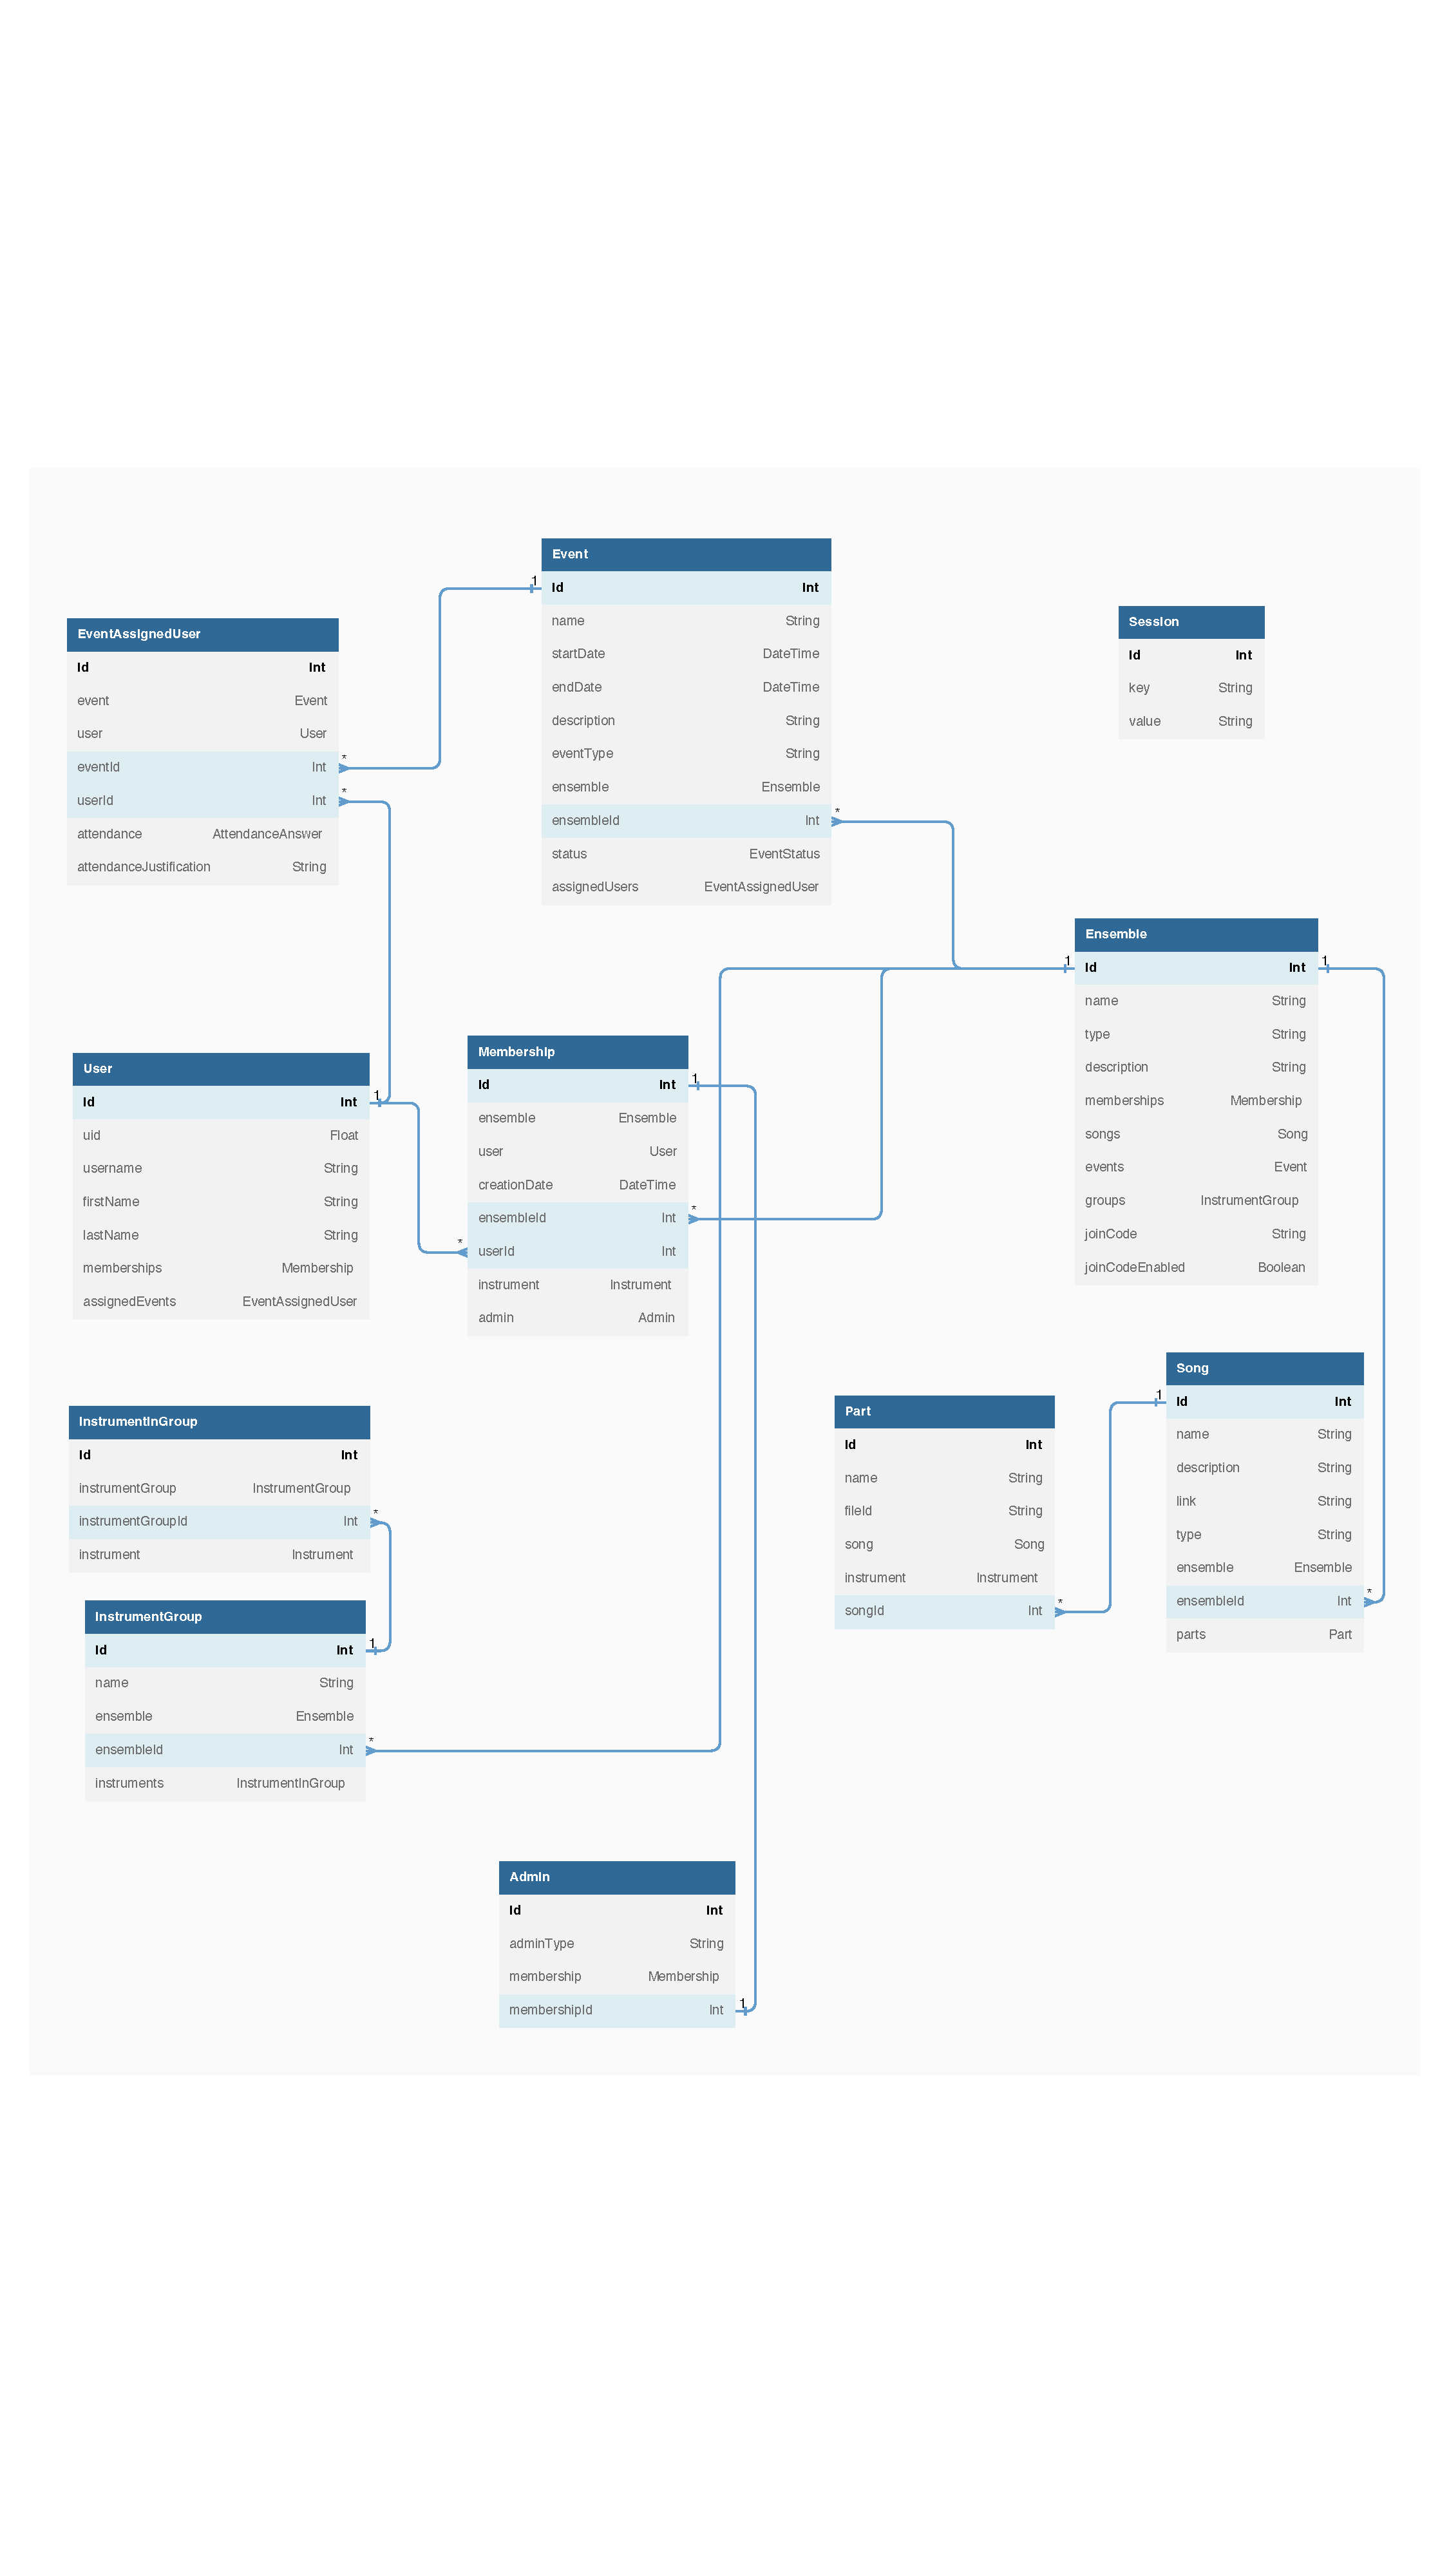
\includegraphics[width=\textwidth]{imagenes/disenyo_tecnico/mordente-db.pdf}
\caption{Modelo de la base de datos}
\label{fig:modeloBaseDatos}
\end{figure}

\section{Arquitectura de Mordente}

Expliquemos la arquitectura del sistema en dos pasos:

\subsection{Arquitectura entre puntos}

Con la arquitectura entre puntos nos referimos a la visualización a alto nivel de las distintas partes físicas necesarias para que nuestra herramienta funcione.

En nuestro caso, existen tres partes claramente diferenciadas:

\begin{itemize}
    \item \textbf{El dispositivo del usuario}, o también llamado cliente. Tiene instalada la aplicación de Telegram, y se comunica bidireccionalmente con los servidores de Telegram para enviar y recibir mensajes.
    \item \textbf{Los servidores de Telegram}. Actúan como intermediarios entre distintos usuarios, así como entre los usuarios y nuestro bot.
    \item \textbf{El bot}. Es un programa que se comunica con los servidores de Telegram para enviar y recibir mensajes, tal y como los clientes, aunque con ciertas diferencias de funcionamiento con los clientes. Este programa puede estar alojado en cualquier ordenador, y en nuestro caso estará alojado en un servidor privado virtual.
\end{itemize}

Esta arquitectura está representada en la figura \ref{fig:arquitecturaPuntos}.

\begin{figure}[h]
\centering
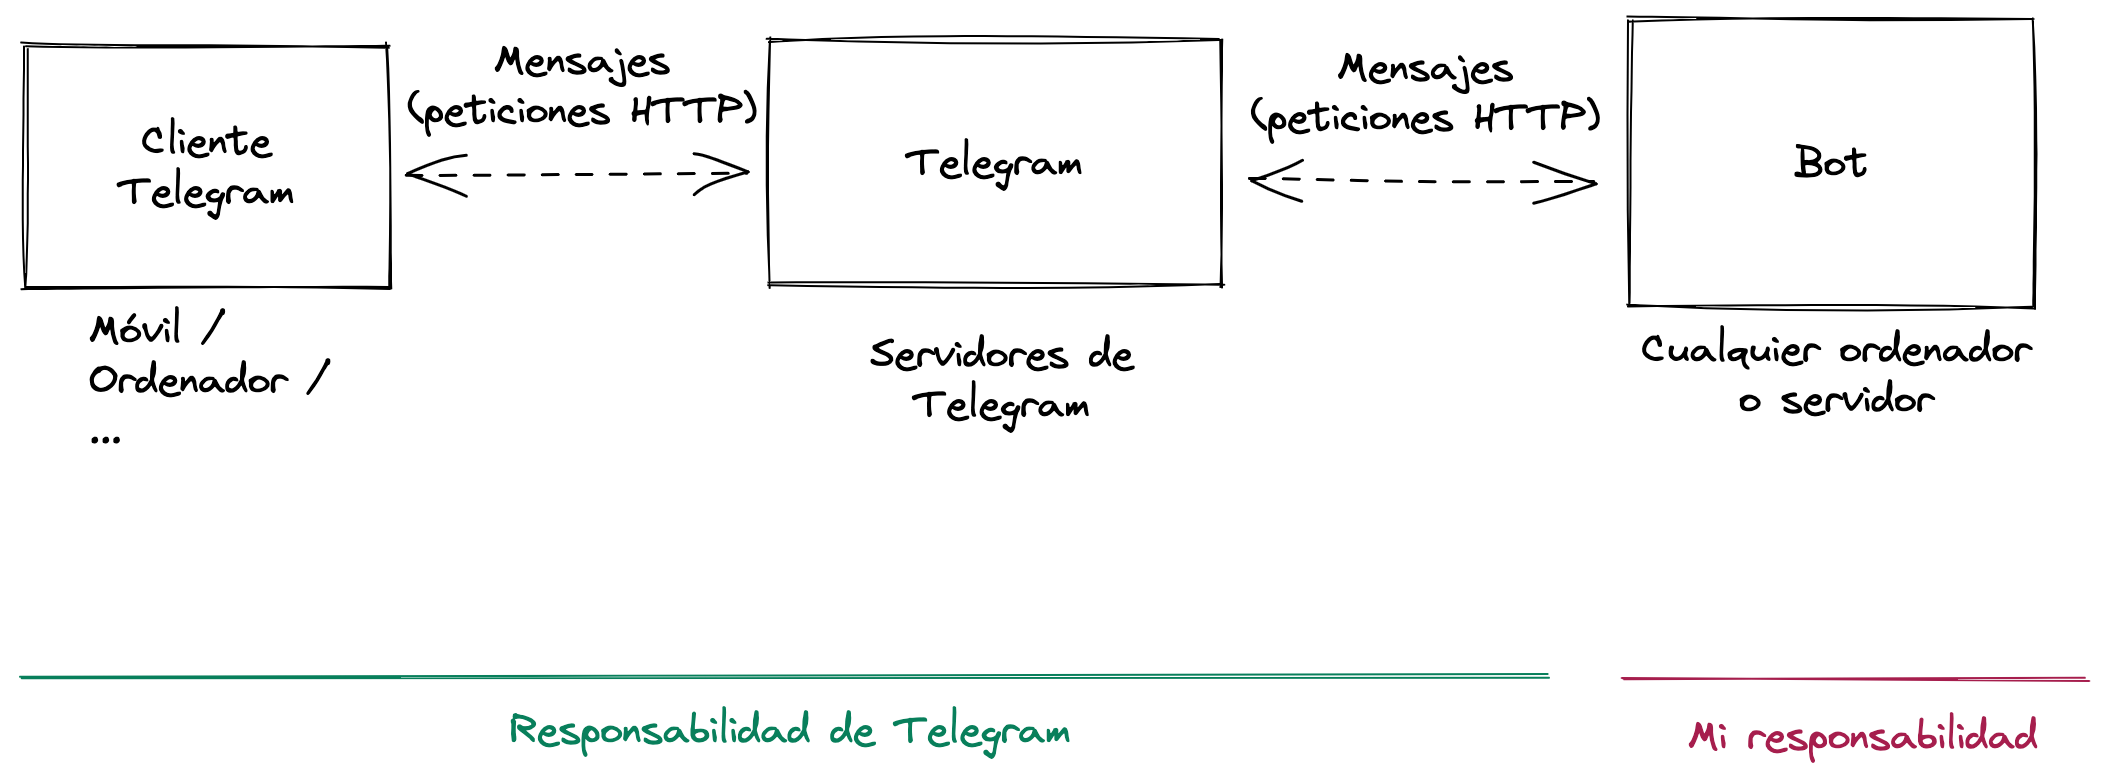
\includegraphics[width=1\textwidth]{imagenes/disenyo_tecnico/arquitectura_puntos.png}
\caption{Arquitectura entre puntos}
\label{fig:arquitecturaPuntos}
\end{figure}

Es importante entender que la única responsabilidad que nos corresponde a nosotros es la de desarrollar la última parte: el bot. El cliente y los servidores de Telegram son partes externas fuera de nuestra responsabilidad, lo cual es una de las ventajas de desarrollar un servicio de este tipo.


% VPS   <->   Telegram API   <->    Telegram Client


\subsection{Arquitectura entre servicios}\label{subsection:arquitecturaServicios}

Para la funcionalidad que necesitamos, el bot debe estar compuesto por varios microservicios a su vez: 

\begin{itemize}
    \item \textbf{El propio bot:} es el microservicio donde implementaremos la comunicación con los servidores de Telegram para recibir mensajes, procesarlos y responderlos adecuadamente.
    \item El bot realiza peticiones a una \textbf{base de datos} donde almacenaremos de forma persistente los datos de los usuarios. Esto garantizará que no perdamos información cuando el bot se reinicie.
    \item Opcionalmente, podremos añadir un microservicio encargado de realizar una \textbf{copia de seguridad} periódica de la base de datos.
    \item Por otro lado tendremos un servicio de \textbf{almacenamiento de archivos} para guardar las copias de seguridad y otros archivos (en nuestro caso, las partituras).
\end{itemize}

En la figura \ref{fig:arquitecturaServicios} se puede visualizar la arquitectura entre los distintos servicios.

\begin{figure}[h]
\centering
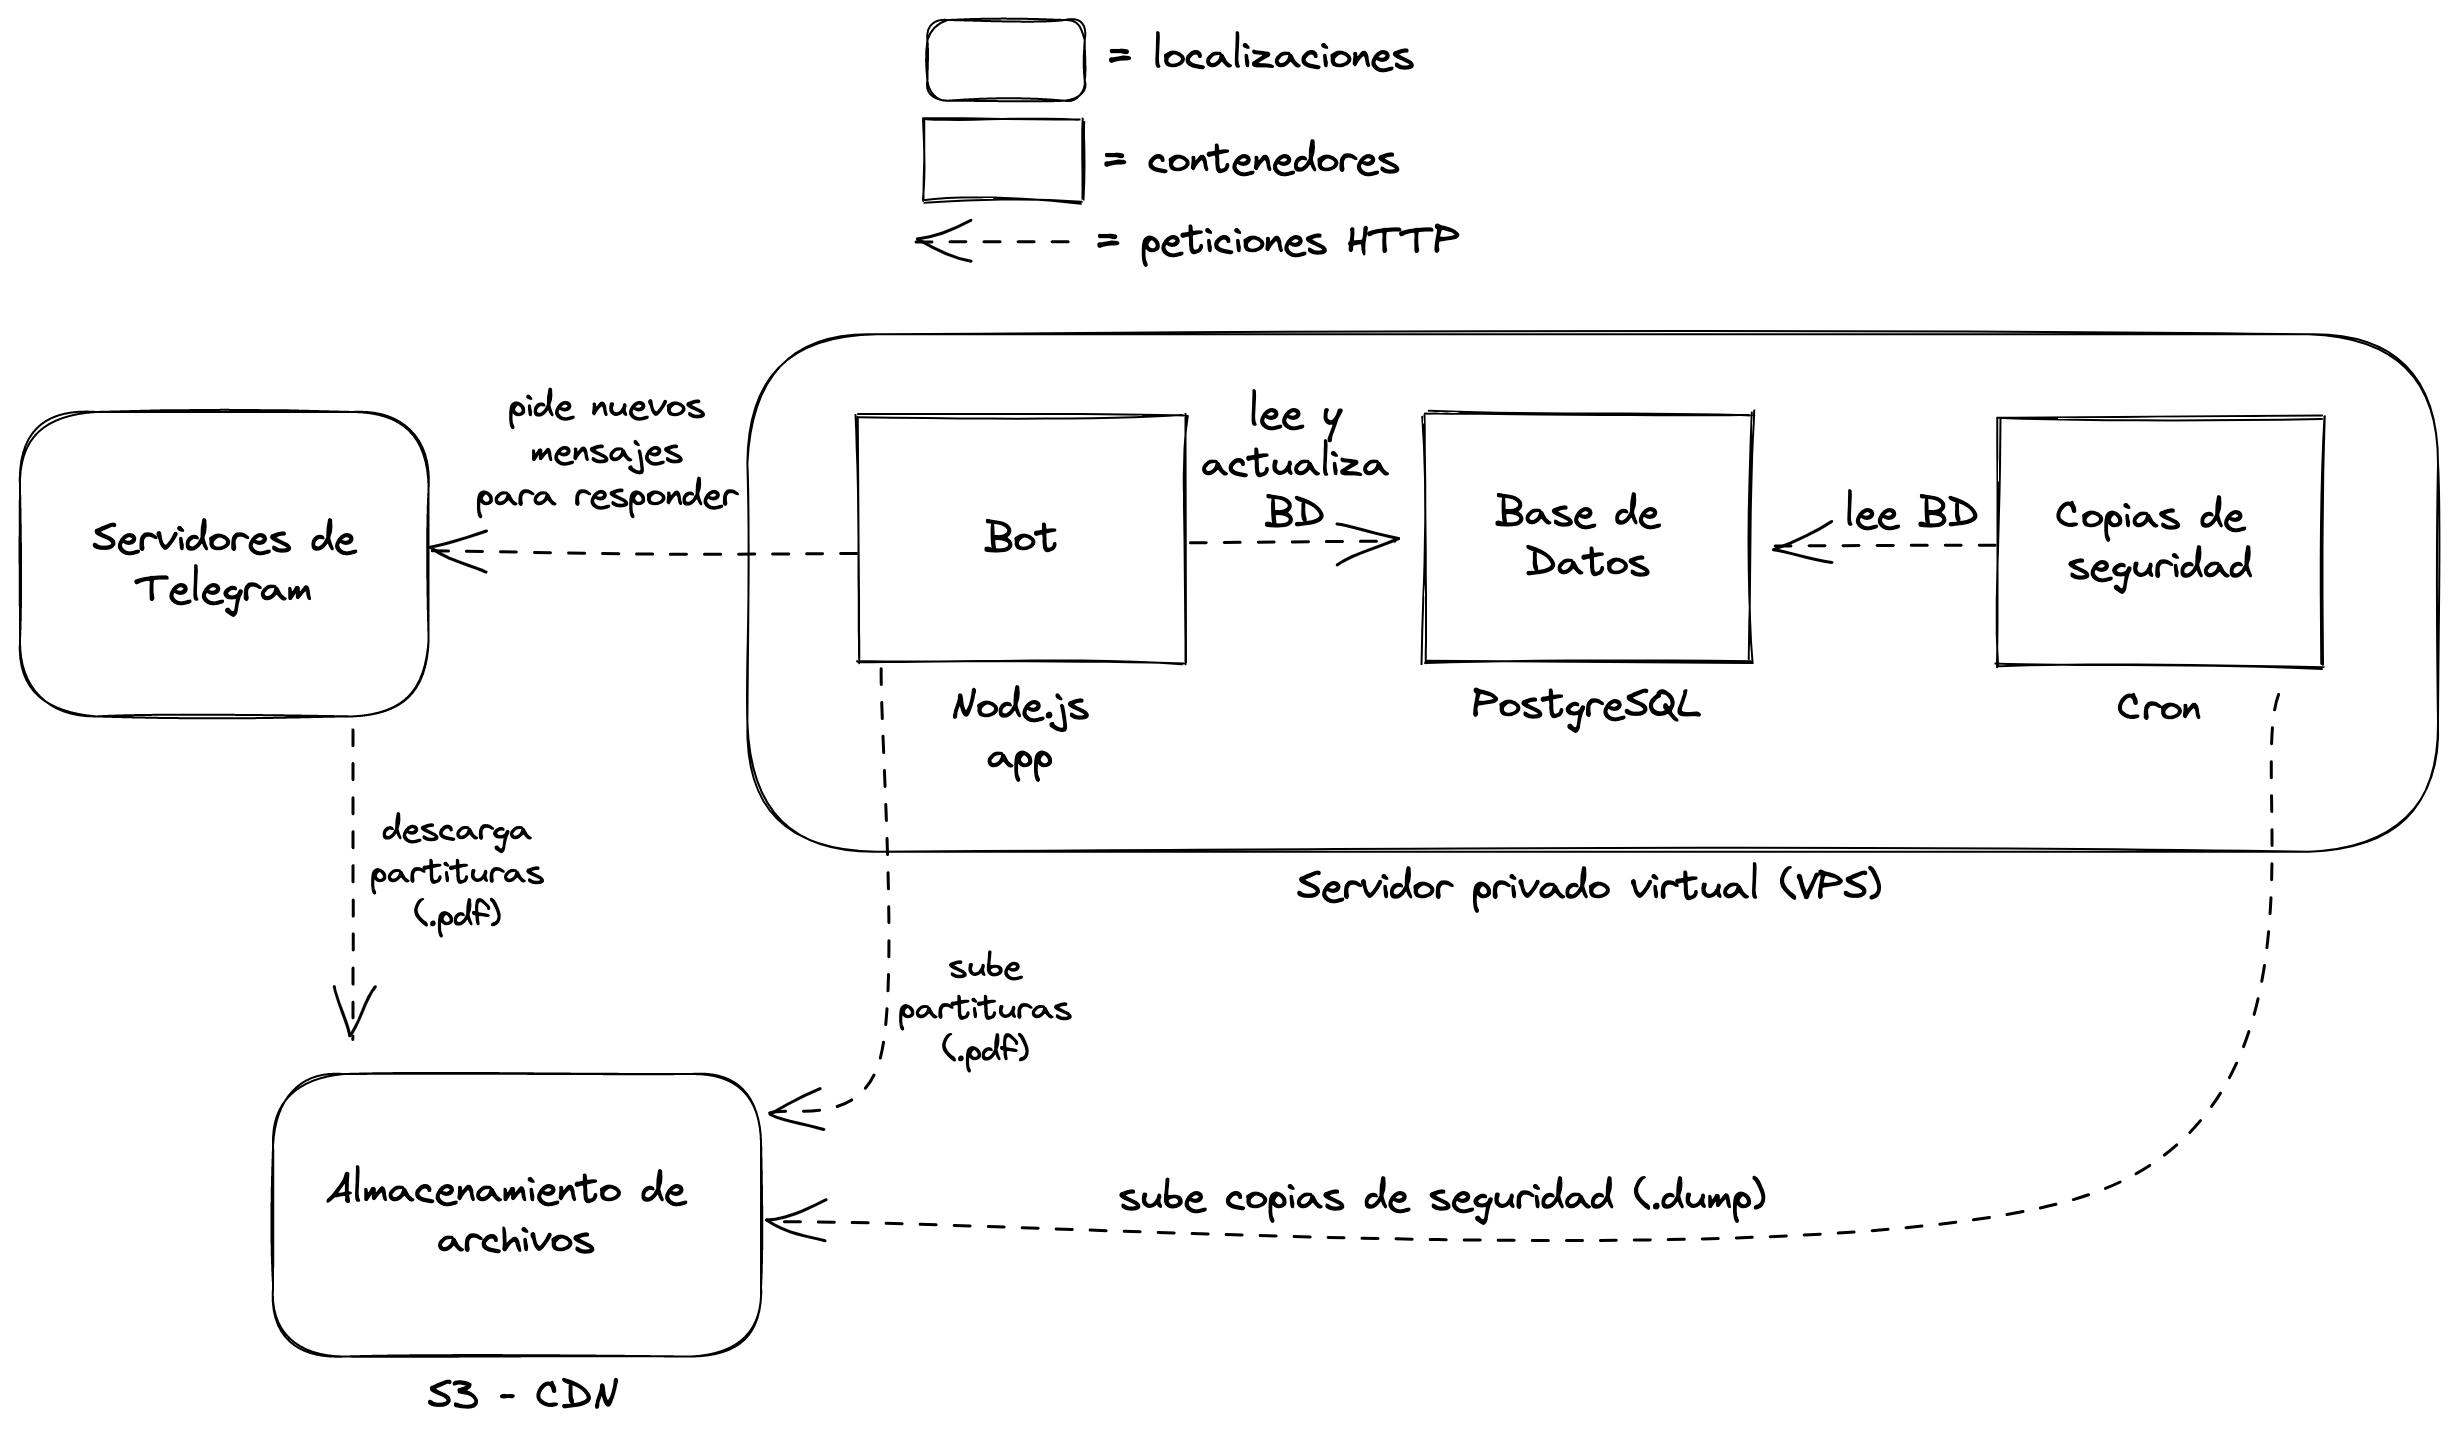
\includegraphics[width=\textwidth]{imagenes/disenyo_tecnico/arquitectura_servicios.png}
\caption{Arquitectura entre servicios}
\label{fig:arquitecturaServicios}
\end{figure}

\subsubsection{Localización de los servicios}

Con respecto a dónde disponer los distintos servicios, existen al menos dos opciones: una es alojarlos en el propio servidor que gestionaremos nosotros y cuyos microservicios podremos levantar en un solo paso usando \textit{Docker Compose}\footnote{\url{https://docs.docker.com/compose/}}, y otra es utilizar servicios auto-gestionados por plataformas externas. Hagamos una reflexión para cada uno de los servicios:

\begin{itemize}
    \item El \textbf{bot} puede estar en un servidor propio o en un servicio gestionado, ambas opciones son válidas. La ventaja de tenerlo en el servidor propio será la mayor cercanía posible con la base de datos, resultando en una mayor velocidad de respuesta. La ventaja de utilizar un servicio gestionado es la mayor facilidad de escalado (mantener la capacidad de respuesta independientemente del número de usuarios), sin embargo esto no es algo prioritario en la primera fase de desarrollo.
    \item Casi todos los proveedores de servicios en la nube ofrecen \textbf{bases de datos} gestionadas\footnote{Ejemplos: Digital Ocean Managed Databases (\url{https://www.digitalocean.com/products/managed-databases}), Heroku Postgres (\url{https://www.heroku.com/postgres}), Google Cloud Firestore (\url{https://cloud.google.com/firestore})}, aunque siempre es conveniente que el bot y la base de datos se encuentren físicamente cercanos para reducir la latencia de las frecuentes consultas. Es por ello y porque no se prevé una gran cantidad de información almacenada durante el periodo inicial que optaremos por alojar la base de datos como un contenedor dentro de nuestro servidor, al igual que el bot.
    \item El \textbf{almacenamiento de archivos} siempre se suele delegar a un servicio externo de almacenamiento de objetos gestionado\footnote{Ejemplos: Amazon S3 (\url{https://aws.amazon.com/es/s3/}), Digital Ocean Spaces (\url{https://www.digitalocean.com/products/spaces}) o Google Cloud Storage (\url{https://cloud.google.com/storage})}. La mayor ventaja de esta aproximación es la disponibilidad de una CDN (\textit{Content Delivery Network}, o Red de Entrega de Contenidos)\cite{whatIsCDN}. Gracias a esta red tendremos un conjunto de servidores distribuidos geográficamente que pueden entregar rápidamente el contenido. Además, usar un servicio fuera de nuestro servidor garantiza que podamos realizar copias de seguridad de la base de datos que no se pierdan si el servidor se rompe por cualquier causa. 
\end{itemize}


\subsubsection{Entorno de producción y de desarrollo}

Es importante tener en cuenta también que esta configuración puede variar dependiendo de si nos encontramos en el entorno de desarrollo o de producción. En nuestro caso, el servicio de copias de seguridad no existirá en el entorno de desarrollo. 

Además, tendremos dos réplicas (una de producción y otra de desarrollo) del bot, la base de datos y el almacenamiento de archivos para que las pruebas no afecten en ningún caso a los datos de los usuarios reales.

\section{Seguridad}

Se intentará maximizar la seguridad de la aplicación gracias a los siguientes puntos:

\begin{itemize}
    \item Los contenedores de Docker utilizados en el servidor están completamente aislados de la red excepto en los puertos que configuremos manualmente. En nuestro caso, el bot podrá conectarse a la base de datos pero ninguno de los contenedores tendrá puertos expuestos al exterior que pudieran ser usados por atacantes.
    \item Gracias al punto anterior, los ataques de denegación de servicio (DDoS) no son un riesgo. Además el servidor tendrá un Firewall configurado.
    \item El uso de herramientas \textit{open-source} como Prisma para hacer las consultas a la base de datos en lugar de realizarlas manualmente con código SQL disminuye al máximo la posibilidad de Inyecciones SQL.
    \item La inyección de código al servidor no es posible ya que no se ejecuta ningún código enviado por el cliente, y por otro lado el cliente es responsabilidad de Telegram.
    \item Se añadirán métodos que permitan detectar automáticamente las vulnerabilidades introducidas por dependencias externas. Como el repositorio estará alojado en GitHub, se propone el uso de \textit{Dependabot}\footnote{\url{https://docs.github.com/es/code-security/dependabot}}.
\end{itemize}


% VPS:

% Telegram API   <->   | app | Postgre | backup |

% Contenedores aislados -> total seguridad
